\setcounter{chapter}{1}         % permet de débuter l'intro à 1. au lieu de 0.
\setcounter{section}{0}
\chapter*{Introduction}         % enlève la numérotation
\phantomsection\addcontentsline{toc}{chapter}{Introduction} % inclus l'intro dans la table des matières
\label{chapter:intro}

La plasticité du \gls{transcriptome} face aux nombreuses perturbations qu'il subit permet à un \gls{organisme} de préserver ses fonctions vitales en tous temps dans une certaine mesure. Par un appel à de nombreux \glspl{mecanisme} de régulation de l'\glspl{genexpr}, les cellules vont alors contrer, compenser ou limiter l'impact de la perturbation. Si les mécanismes majeurs de la régulation ont pu être identifiés dès les premières quantifications de l'expression, le récent développement des technologies de \gls{transcriptomique} a permis d'accélérer cette tendance. La recherche en médecine moléculaire s'est donc emparée de cet outil dans une démarche d'identification systématique de la \gls{fonction_biologique} de gènes encore mal connus ou de la cause de leur implication dans une maladie, un \gls{phenotype} ou une \gls{condition}.

La quantité de données faisant, le besoin de méthodes d'analyse biostatistique capables de gérer autant d'information pour en ressortir des biomarqueurs, caractéristiques spécifiques et mesurable d'une condition, s'est accru. C'est dans ce contexte qu'on a vu l’essor des méthodes d'analyse par réseau en biologie \cite{Barabasi2004} et plus particulièrement celles dites de réseau de co-expression de gènes qui reposent sur la synchronisation de l'expression entre gènes. Par leur capacité à saisir l'ensemble des variations les plus subtiles dans le \gls{transcriptome} et les variations conjointes entre gènes, les réseaux de co-expression de gènes ont su montrer leur intérêt dans la recherche de biomarqueurs de maladies complexes et encore mal comprises telles qu'Alzheimer \cite{Hu2020Nov} ou le cancer du sein \cite{Garcia-Cortes2020Jul}. Pourtant, leur emploi reste encore limité aux équipes possédant l'expertise d'un·e bio-informaticien·ne, retardant leur potentiel pour l'étude de nombreux phénomènes. Parmi eux, le vieillissement y gagnerait pourtant à utiliser des approches par réseau. De nature complexe, le vieillissement est un phénomène qu'on résume encore trop souvent à sa seule composante de sénescence. Il est pourtant le résultat de nombreux mécanismes entrecroisés que la co-expression est à même de décomposer grâce à son étude à l'échelle d'un système et pas seulement de ses acteurs individuels, les gènes.

Les travaux réalisés durant ce doctorat ont donc été divisé en deux parties avec un but chacune. Premièrement, tester la pertinence du développement d'un outil d'architecture pipeline modulaire, sous forme de paquet R, contenant une aide à l'interprétation et visant à pérenniser l'analyse de co-expression de gènes au vu de l'évolution des méthodes pour la réaliser. Deuxièmement, évaluer le potentiel de découverte de l'analyse de co-expression de gènes à travers différents tissus et tranches d'âge pour une meilleure compréhension du vieillissement humain en priorisant des gènes.

Cette introduction vise à donner les clefs essentielles à la compréhension des différents concepts biostatistiques, bio-informatiques et médicaux employés tout au long de cette thèse. Elle est suivie par deux chapitres dont le premier est la présentation de l'outil GWENA dédié à l'analyse de réseaux de co-expression de gènes et de son application sur l'étude du vieillissement du muscle squelettique. Le second chapitre est une étude à plus large spectre du vieillissement analysant les \glslink{fonction_biologique}{fonctions} communes et spécifiques du vieillissement à travers 10 tissus humains. S’ensuivent une conclusion résumant les apports de mes travaux, puis une discussion les replaçant dans le contexte des connaissances actuelles et les perspectives futures dans ce domaine.




\section{La complexité du vivant}

\subsection{Un fonctionnement multiple issu d'un code unique}

\begin{figure}[b]
    \centering
    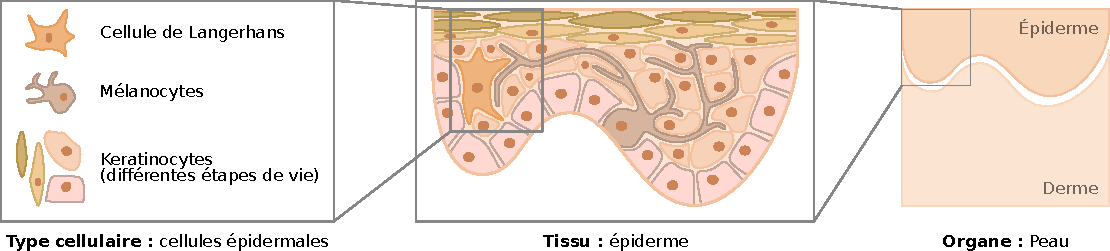
\includegraphics[width=\textwidth]{img/intro/1_context/intro_1_cell_tissue_organ.pdf}
    % \caption{Exemple d'agrégation de différents types cellulaires issus de l'épiderme en tissu puis des ti}
    \caption[Différentes échelles de visualisation de l'organisation cellulaire avec l'exemple de la peau.]{Différentes échelles de visualisation de l'organisation cellulaire avec l'exemple de la peau. Les cellules majoritairement présentes sont les kératinocytes responsable de la fonction barrière, les mélanocytes responsables de la protection solaire notamment, et les cellules de Langerhans responsables d'une fonction immunitaire primaire}
    \label{fig:intro_tissu_type_cellulaire}
\end{figure}

Le vivant est fait d'une diversité d'\glspl{organisme} à l'image de sa complexité. Chacun de ces organismes est composé d'une ou plusieurs \textbf{cellules} œuvrant ensemble pour la survie et la reproduction de celui-ci. Ces êtres multicellulaires sont bien souvent constitués d’une association de cellules à la \glslink{fonction_biologique}{fonction} et la forme bien différentes de ses voisines. Ainsi, chez des organismes constitués d'un très faible nombre de cellules comme les Myxozoa constitués au maximum de 7 cellules \cite{Morris2010Aug} tout comme chez des organismes de taille bien plus importante comme l'humain fait d'entre 10\textsuperscript{12} et 10\textsuperscript{16} cellules \cite{Bianconi2013}), on retrouve des cellules spécialisées pour une tâche spécifique \cite{Panina2020Sep} (Figure \ref{fig:intro_tissu_type_cellulaire}). Celles-ci servent différents objectifs tels que la protection, l'acheminement d'éléments nutritifs, ou encore la transmission de matériel génétique. Chez l’humain, ces cellules seront par exemple respectivement des kératinocytes \cite{Yuki2007Apr}, des cellules endothéliales de l’intima \cite{Yuan1991Aug}, des ovocytes \cite{Trounson2013}. En s’assemblant entre cellules de même type, puis en formant des complexes avec d’autres \glspl{type_cellulaire}, les organismes parviennent à former alors des structures nommées \textbf{\gls{tissu}} \cite{Hekselman2020Mar} qui elles-mêmes assemblées vont former un \gls{organe}. La combinaison de kératinocytes, de mélanocytes, de cellules de Langerhans et les cellules de Merkel connectées par une matrice extra-cellulaire forment ainsi le tissu épidermal, ou plus simplement l’épiderme \cite{Bettley1965}.

Pour effectuer chacune de ces tâches spécialisées, les différents types de cellules vont produire en partie des \textbf{protéines} ayant des fonctions biologiques différentes de leurs voisines. Bien qu'il existe une très large diversité de fonctions, 32 catégories de fonctions selon le projet Gene Ontology \cite{Ashburner2000}, on peut toutefois les regrouper en 3 familles de fonctions majeures \cite{Mathews2012}:  
\begin{itemize}
    \item \textbf{les fonctions catalytiques} : les protéines, dans ce cas appelées enzymes, présentent une activité d'augmentation du taux de réaction chimique en diminuant l'énergie d'activation nécessaire. Ces enzymes sont spécifiques d'une transformation d'un substrat vers un produit. Elles peuvent cependant voir leur fonction altérée par des activateurs (co-facteurs, co-enzymes) et des inhibiteurs (co-répresseurs). Par exemple, l'alcool déshydrogénase va, avec la liaison du coenzyme NAD+ et d'un cofacteur zinc, catalyser l'oxydation d'alcools en aldéhydes ou cétones.
    \item \textbf{les fonctions de signalisation ou liaison} : en se fixant à un récepteur ou en étant un récepteur à la fixation d'un ligand, les protéines permettent de faire transiter de l'information en intra ou extra cellulaire. La fixation entraîne la transmission d'un signal physique ou chimique via une cascade d'événements qui vont conduire à une réponse cellulaire. Par exemple, la production d'une protéine d'insuline par le pancréas va, en se fixant sur les récepteurs membranaires des cellules, déclencher des \glspl{mecanisme} de stockage du glucose. Ceci se traduit dans le foie par l'initiation de la transformation du glucose en glycogène.
    \item \textbf{les fonctions de structuration} : les protéines par leur forme et propriétés physico-chimiques hautement modulables permettent de donner une architecture ou des propriétés mécaniques aux cellules dans/autour desquelles elles se trouvent. Par exemple la combinaison de protéines de myosine II et d'actine permettent la contraction musculaire par des phénomènes de glissement de ces protéines.
\end{itemize}

Pour être produites, ces protéines suivent chacune un plan de construction défini grâce au code génétique comportant 4 unités, des nucléotides : adénosine, tyrosine, guanine et cytosine. Ils s'enchainent dans une séquence qui va encoder l'information génétique d'un individu et forment un polymère de longueur variable nommée Acide DesoxyRibonucléique (ADN). Cette molécule d'ADN, identique dans chacune des cellules d'un organisme, est découpée en plusieurs chromosome. Cette molécule d'ADN est présente à l'identique dans chacune des cellules d'un organisme et encode au long de sa séquence l'information relative aux protéines sous forme d'unité nommée \textbf{gène}. Chez l'humain sur qui on se concentrera dans ce manuscrit, la version 37 de l'annotation du génome humain du projet GENCODE \cite{Frankish2019Jan} considère ainsi qu'il existe 60 651 gènes. Cependant, tous parmi eux ne produisent pas de protéine. On distingue en réalité les gènes dits \textbf{codants} (19951 toujours dans GENCODE 37) car produisant des protéines et les gènes \textbf{non-codants} qui codent en fait d'autres entités moléculaires que des gènes, mais tout aussi utiles à la cellule.

Chez l'humain et plus généralement les eucaryotes, l'ADN est contenu dans le noyau de la cellule où il se trouve condensé après plusieurs étapes de repliement à l'aide de protéines appelées histones. La machinerie cellulaire de production des protéines étant située à l'extérieur du noyau, une étape intermédiaire de transcription est nécessaire afin de copier la séquence ADN d'un gène sous la forme d'une molécule capable de sortir du noyau : l'ARN messager (ARNm). Semblable à l'ADN, l'ARNm est cependant monobrin alors que l'ADN est double brin. Dans cette molécule, la thymine est remplacée par un autre nucléotide, l'uranine. La taille d'un brin d'ARNm est par ailleurs plus petite que celle d'un fragment d'ADN car il embarque l'information correspondant à un gène seulement. Chacun des triplets de nucléotides sur sa séquence, appelés codons, encode pour un des 20 types d'acides aminés constituant la protéine associée (Figure \ref{fig:intro_code_genetique}).

\begin{figure}[hb]
    \centering
    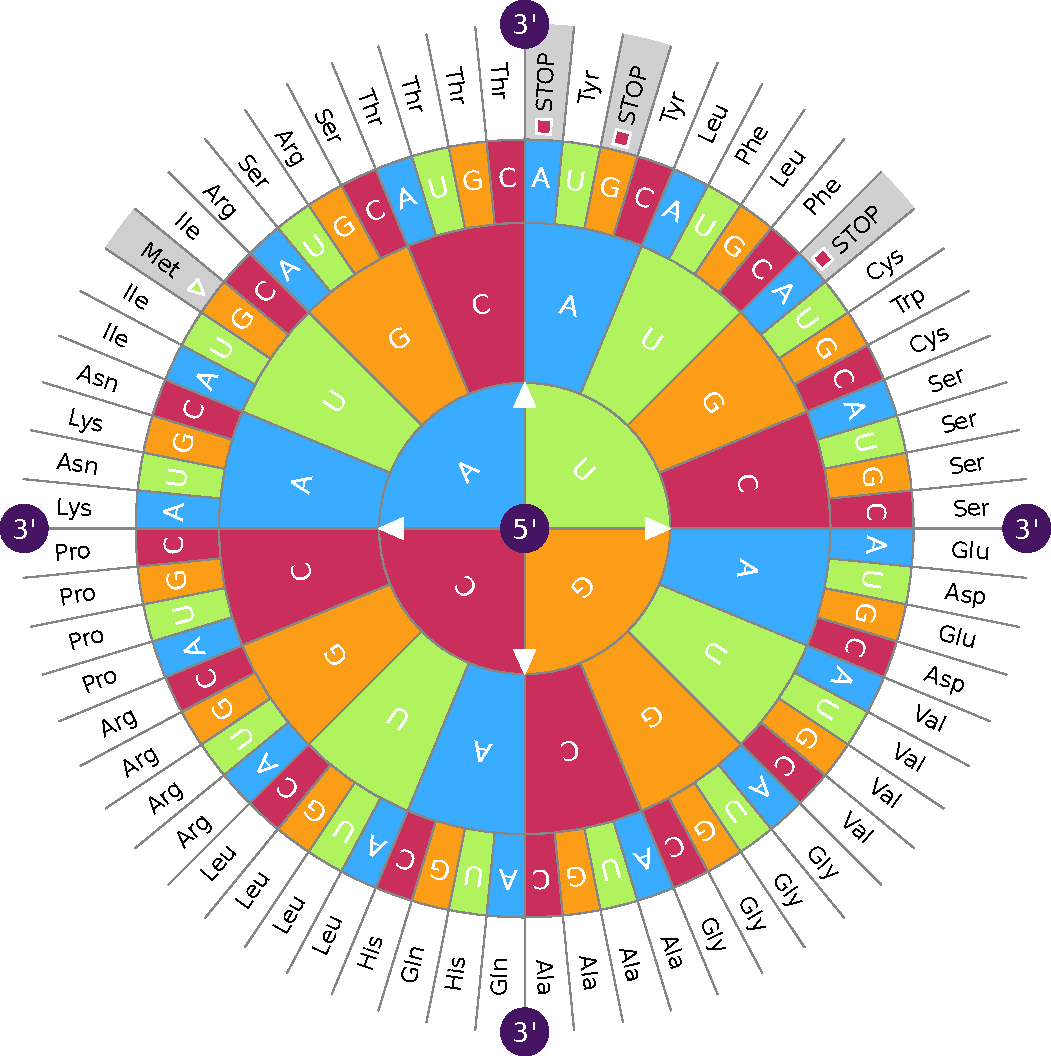
\includegraphics[width=0.9\textwidth]{img/intro/1_context/intro_1_code_genetique.pdf}
    \caption[Correspondance des codons avec l'acide aminé produit.]{Correspondance des codons avec l'acide aminé produit. La lecture s'effectue du centre du cercle vers l'extérieur pour respecter le sens 5' \textrightarrow{} 3' de l'ARN. Le codon de la méthionine qui est le codon de départ de toute traduction est indiqué par un triangle vert, et les trois codons stop sont indiqués avec un carré rouge.}
    \label{fig:intro_code_genetique}
\end{figure}


Une fois copié depuis l'ADN, l'ARNm immature, composé de sous unités appelées introns et exons, sort du noyau vers le cytoplasme pour subir une étape de maturation. Durant celle-ci, il se voit retirer ses introns et certains exons ou sections d'exons selon les besoins de sous-fonction de la protéine finale. On nomme \textbf{\glspl{transcrit}} ces différentes versions d'ARNm issues d'un même gène (Figure \ref{fig:alternative_splicing}). Ainsi, on considère que la transcription d'un gène sous n'importe lequel de ses transcrits correspond à l'expression de son gène dans un échantillon. Par la suite, une étape de traduction de l'ARNm en une séquence d'acides aminés donnera une molécule qui sera la base de la protéine. Après le repliement de ce polymère et des modifications dites post-traductionnelles par la machinerie cellulaire, la protéine sera enfin opérationnelle pour réaliser la fonction qui lui incombe. 

\begin{figure}[hb]
    \centering
    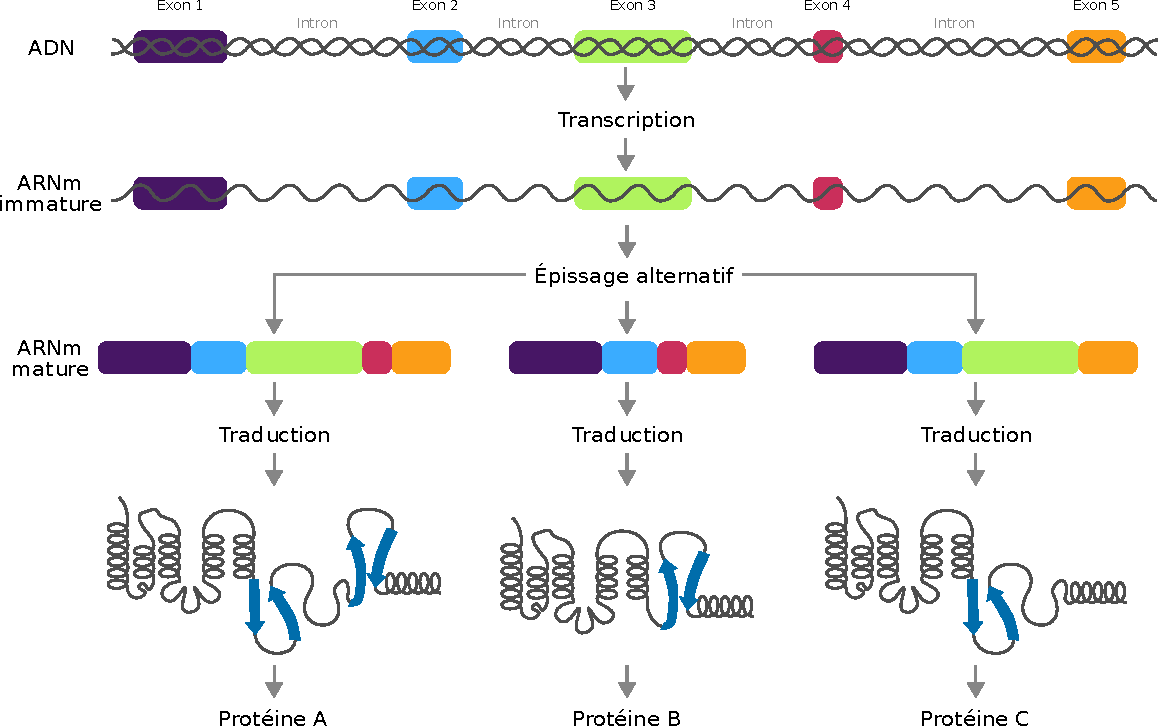
\includegraphics[width=\textwidth]{img/intro/1_context/intro_1_alternative_splicing.pdf}
    \caption{Épissage alternatif avec un exemple sur 5 exons et 3 protéines différentes pouvant donc résulter du même ARNm.}
    \label{fig:alternative_splicing}
\end{figure}

\subsection{La régulation de l'expression pour une spécification cellulaire}

Comme mentionné précédemment, l'ADN est identique dans toutes les cellules d'un \gls{organisme}, alors même que chaque cellule n'est capable d'exprimer, de transcrire, que les gènes spécifiques à sa fonction. Les myocytes seront par exemple les cellules majoritaires à produire de la myosine et les kératinocytes seront les cellules majoritaires à produire de la kératine. Cette capacité de production spécialisée des cellules est permise par les différents \glspl{mecanisme} de régulation de l'\glspl{genexpr} (et par extension leur répression) qui sont établis dès les premières différenciations cellulaires au cours du développement d'un organisme. Tous ces mécanismes, dits de régulation, sont interconnectés pour ajuster en temps réel la quantité de protéines nécessaires au fonctionnement immédiat de la cellule \cite{Weake2010Jun}. On distingue les mécanismes suivants : 
\begin{itemize}
    \item \textbf{La régulation de l'initiation de la transcription} : lors de la transcription de l'ADN d'un gène en ARNm, l'accessibilité des régions à transcrire dépend de l'impact de plusieurs éléments de régulations parmi lesquels on retrouve les amplificateurs (en anglais \textit{enhancers}) et les inactivateurs (en anglais \textit{silencers}), des séquences riches en motifs de liaison de facteurs de transcription capables respectivement d'augmenter ou diminuer le niveau d'expression de gènes \cite{Levo2014Jul}. Très souvent présents dans des boucles de rétro-action, ces facteurs de transcription qui sont des protéines peuvent eux-mêmes voir leur expression augmentée ou diminuée par des acteurs variés tels que des ARN non-codants et des protéines \cite{Chen2020May}.
    \item \textbf{La conformation de la chromatine} : pour rentrer dans l'espace que représente le noyau d'une cellule, l'ADN doit être replié sur lui-même à l'aide de protéines telles que des histones. Cette condensation de l'ADN implique de rendre spatialement disponibles certaines régions à la transcription et indisponibles d'autres \cite{Kadauke2009Jan}.
    La variation d'accessibilité de ces régions est notamment due à la localisation des boucles que forme la chromatine avec elle-même.
    \item \textbf{La modification post-transcriptionnelle} : les ARNm nécessitent l'ajout d'une 7-methylguanosine sur l'extrémité 5' (coiffe 5'), un épissage et une polyadénylation sur l'extrémité 3' (ajout d'une queue poly A) afin d'être traduits en protéine. En l'absence de ces modifications, les ARNm sont détruits par la cellule \cite{Mercer2010Nov}.
    \item \textbf{La méthylation} : les îlots CpG sont des structures de l'ADN où une cytosine est suivie d'une guanine dans le sens 5' \textrightarrow{} 3'. Très présents dans les régions d'initiation de la transcription, ils peuvent subir l'ajout d'un groupement méthyl empêchant la fixation de différents agents de la transcription \cite{Gutierrez-Arcelus2013Jun}.
    \item \textbf{La susceptibilité à la dégradation} : afin de perdurer plus de quelques minutes dans la cellule, certains ARN contiennent ou évitent des motifs de nucléotides influant la vitesse de dégradation (éléments riches en AU, codon stop prématuré, taille de queue poly-A) \cite{Yu2001}. Des ARN non-codants tels que les ARN interférents de petite taille (ARNip), les ARN micro (ARNmi) et les ARN longs non codants (ARNlnc) peuvent également favoriser la dégradation de certains ARN cibles \cite{Patil2014Jan}.
    \item \textbf{La régulation de la traduction} : en perturbant l'initiation, l'élongation ou la terminaison de la traduction des ARNm, des acteurs tels que les fragments dérivés d'ARN de transfert (ARNt) \cite{Krishna2021Mar}, le niveau de ribosomes disponibles \cite{Khajuria2018Mar} ou encore des ARNmi \cite{Meijer2013Apr}.
\end{itemize}


% \todo[inline]{Figure mixée de celle de ZaZo0o et celle trouvée}
%  https://www.sciencedirect.com/science/article/pii/S0167488916302919
%% TRANSITION : parler des erreurs/variabilité biologique ? 


\subsection{L'étude de l'expression des gènes pour la résolution de conditions cliniques}

Qu'il s'agisse du génome entier, du génome de tissus ou du génome de cellule spécifiques, les études de profilage des transcrits produits, ou \textbf{\gls{transcriptome}}, ont permis de mieux comprendre le fonctionnement basal et sain de ces entités \cite{Hughes2000, Cloonan2008Jul}. Aussi appelées approches systématiques, ces études servent en premier lieu à identifier de gènes impliqués dans des fonctions physiologiques (annotation) \cite{Munji2019Nov}, à associer des régions de l'ADN à des traits quantitatifs (locus de caractère quantitatif LCQ ou en anglais QTL) \cite{Sarkar2019Apr}, ou encore à identifier des \glspl{mecanisme} de régulation de la transcription \cite{Segales2016Dec} ou des mécanismes cellulaires tels que la différenciation \cite{Godoy2018Jul}, la réparation de l'ADN \cite{Jividen2018Dec}, etc. De plus en plus de ces études permettent par la suite une réutilisation de ces données en les déposant dans des répertoires en ligne tels que Gene Expression Omnibus (GEO) \cite{Barrett2013Jan} et ArrayExpress \cite{Athar2019Jan}. Ils ont notamment été utilisées pour créer Expression Atlas \cite{Lukk2010Apr}, une carte globale d'\glspl{genexpr} avec une mise à jour récente pour inclure des données provenant du séquençage de cellules uniques \cite{Papatheodorou2020Jan}. Ces données, ainsi que la connaissance associée par les études dont elles sont issues, permettent alors d'avoir une vision générale du fonctionnement sain de l'humain pour mieux étudier par contraste les perturbations qui ont lieu.

Ces perturbations du fonctionnement cellulaire peuvent provenir de différentes \glspl{condition} telles qu'une maladie, une mutation, un stress, ou encore l'âge. Avec chacune d'elle, la régulation de l'expression se retrouve altérée différemment par rapport au fonctionnement sain. Le transcriptome, ensemble des ARN ou transcrits produits, est alors un témoin direct des fonctions mises en défaut \cite{Morozova2009Aug}. L'étude de la quantité de chaque transcrit exprimé donne ainsi un moyen direct de comprendre l'origine de manifestations macroscopique telles que la présence de tumeur ou nécrose dans les tissus \cite{Pennycooke2001Jan,Ahn2018Apr}. Ce type d'étude permet également une compréhension plus fine des variations moléculaires telles que des variations de pH ou la mauvaise absorption de nutriment dans l'\gls{organisme} \cite{Martin2017Jun,Ventura2020Nov}. En recherchant les transcrits dont la quantité change significativement entre une personne saine et une personne affectée par la condition considérée, il est alors possible d'isoler des biomarqueurs de la condition en question. Outre leur rôle d'aide au dépistage de certaines conditions, les biomarqueurs ont un intérêt en termes de soin car ils peuvent représenter ce qu'on nomme une cible thérapeutique \cite{Collins2017Jan}. En conceptualisant des molécules en fonction du biomarqueur, on peut être capable d'interférer avec le biomarqueur, ses précurseurs, ses co-acteurs ou ses produits, le tout en vue de limiter leurs potentiels impacts négatifs. La détection fiable de ces biomarqueurs est alors primordiale et dépend tant de la méthode de quantification des transcrits que de leur analyse.

%% Sources d'aide à la rédaction
% https://www.mdpi.com/1422-0067/18/8/1652/htm#B4-ijms-18-01652 : Transcriptome Profiling in Human Diseases: New Advances and Perspectives
% Intro utile pour retravailler cette section : https://www.nature.com/articles/nrg.2017.96

%% Infos potentiellement rajoutables :
% - On s'est intéressés tardivement au transcriptome historiquement car on pensait que tout le non codant était du "junk DNA". Ça a changé avec l'arrivée en 2000 du premier génome humain (https://www.ncbi.nlm.nih.gov/pubmed/5065367/). Formulation "De la première version du génome humain dans les années 2000 à sa dernière version complète en 2021, l'analyse du génome humain a permis de désavouer l'hypothèse du junk DNA. On ne considérant plus le génome non-codant comme inutile, l'étude du transcriptome au complet a permis de nombreuses perspectives d'études sur des conditions cliniques alors dans une impasse.

\section{Les technologies de transcriptomique pour la quantification de l'expression des gènes}

\subsection{Historique des technologies de transcriptomique}

L'ARN est une molécule dont la stabilité est faible et la dégradation rapide en raison des nombreuses enzymes de dégradation la ciblant dans une cellule. Les premières technologies de \gls{transcriptomique} ont donc rarement ciblé les ARN en eux-mêmes et ont plutôt construit des ADN complémentaires (ADNc) de leurs séquences à l'aide de transcriptases inverses découvertes en 1970 \cite{Temin1970Jun}. Ces premières technologies furent basées sur les marqueurs de séquence exprimée (\textit{expressed sequence tags} en anglais ou EST), de courtes séquences d'ADNc identifiantes de transcrits qu'on détectait ensuite par migration sur gel. Développés au début des années 70, les EST ont servi de base à la méthode SAGE (\textit{Serial Analysis of Gene Expression}) créée en 1995 \cite{Velculescu1995Oct} qui analyse les EST concaténés via le séquençage Sanger lui-même inventé en 1975 \cite{Sanger1975May}. Cette technique de séquençage alors très populaire à l'époque \cite{Marra1998Jan} est dite rétrospectivement de bas débit et a permis les premiers séquençages de \glspl{transcriptome} partiels \cite{Jeppesen1970Apr} ou complets pour des \glspl{organisme} à ARN de petite taille comme le bactériophage MS2 \cite{Fiers1976Apr}. La quantification par réaction en chaine d'ARN retro transposé (RT-qPCR de l'anglais \textit{reverse transcription quantitative polymerase chain reaction}) combinée à un buvardage de northern\footnote{Traduction issue de \url{http://gdt.oqlf.gouv.qc.ca/ficheOqlf.aspx?Id_Fiche=8392423}} (en anglais \textit{northernblot}) fut également utilisée à partir de la fin des années 80 en raison de sa grande précision\cite{Becker-Andre1989Nov}.

L'utilisation de SAGE et de RT-qPCR dans l'étude de l'\glspl{genexpr} a toutefois diminué au profit de nouvelles technologies capables de quantifier un plus grand nombre de transcrits simultanément \cite{Lowe2017May}. Les puces à ADN par hybridation (en anglais \textit{hybridization-based microarrays}) ont ainsi été prisés dès le milieu des années 90 \cite{Schena1995Oct} après la commercialisation de la première puce Affimetrix \cite{Lenoir2006} en raison de leur faible rapport coût sur transcrits quantifiés. Cependant, face à la contrainte des puces à ADN de devoir connaître les séquences des transcrits à quantifier, la technologie du RNA-seq  (séquençage de l'ARN, \textit{RNA sequencing} en anglais) est devenue un incontournable dans nombre d'études. 
Profitant de l'amélioration des technologies de séquençage génomique via toujours une transcription inverse de l'ARNm en ADNc, la technologie du RNA-seq va émerger dans les années 2000 et est annoncée comme révolutionnaire \cite{Wang2009Jan}. Toutefois, sa mention dans une publication n'arrivera qu'en 2008 \cite{Nagalakshmi2008Jun} bien qu'elle soit utilisée dès 2006 \cite{Cheung2006Dec}.

Les puces à ADN et le RNA-seq sont encore aujourd'hui les deux technologies de quantification de l'expression des gènes utilisées, malgré le déclin annoncé des puces à ADN (Figure \ref{fig:intro_count_by_year_rnaseq_microarray_est}). Les bio-informaticien·ne·s sont donc amené·e·s à devoir traiter et analyser les données issues de ces deux approches en tenant compte des propriétés biologiques, techniques et statistiques respectives à chacune des deux technologies.

\begin{figure}[ht]
    \centering
    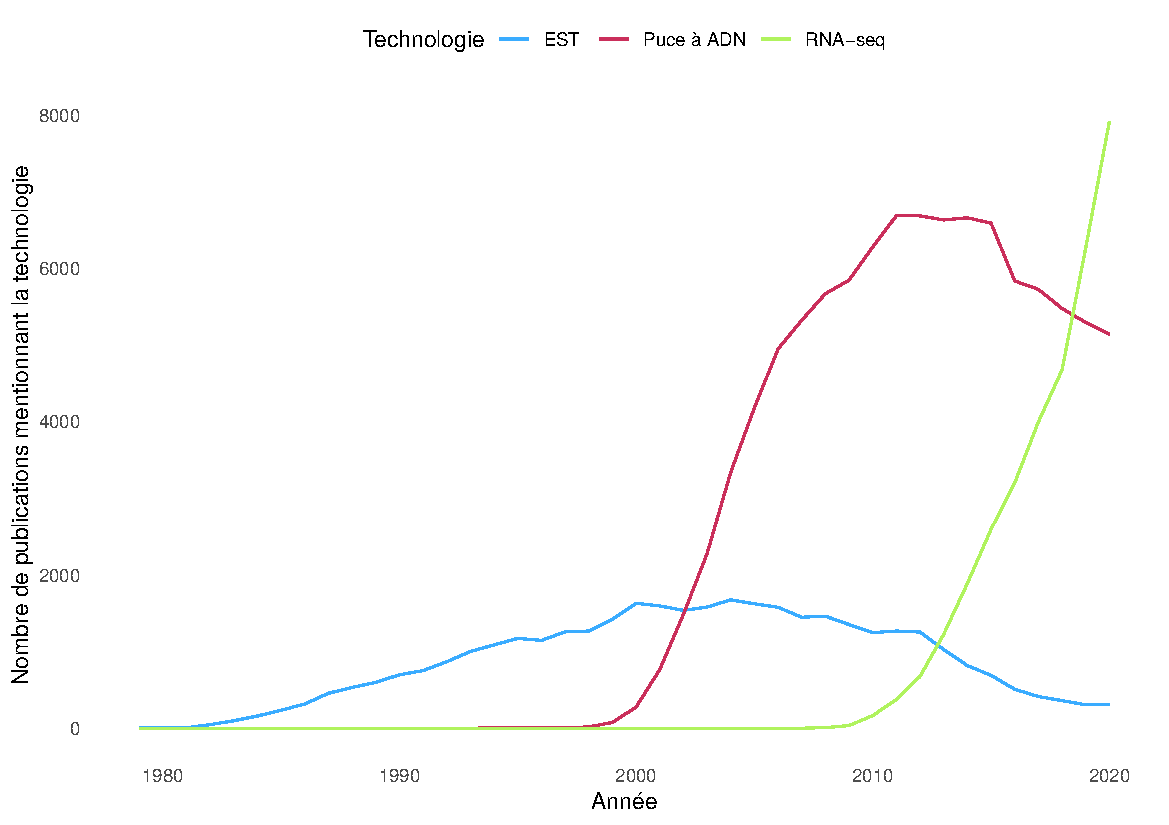
\includegraphics[width=\textwidth]{img/intro/2_meth_transcripto/intro_2_count_by_year_rnaseq_microarray_est.pdf}
    \caption[Évolution de l'utilisation des différentes techniques de transcriptomique en se basant sur le nombre de publications les mentionnant]{Évolution de l'utilisation des différentes techniques de transcriptomique en se basant sur le nombre de publications les mentionnant. Les résultats proviennent du site PubMed (\url{https://pubmed.ncbi.nlm.nih.gov}) avec les requêtes suivantes : \textbf{EST} = "cDNA library" OR "cDNA libraries" OR "complementary DNA library" OR "complementary DNA libraries" OR "expressed sequence tag" OR "expressed sequence tags", \textbf{Puce à ADN} = "micro array" OR "microarray" NOT "chromosomal", \textbf{RNA-seq} = "RNA Seq" OR "RNA-Seq" OR "RNASeq".}
    \label{fig:intro_count_by_year_rnaseq_microarray_est}
\end{figure}



%% Sources d'aide à la rédaction
% Un TRES bon site sur les technos de sequencage : http://education.knoweng.org/sequenceng/

%% Infos potentiellement rajoutables :
% - L'importance et l'impact du projet de séquençage du génome humain sur les technologies de séquençage avec les retombée bénéfique pour la transcriptomique :  invalidation de l'idée de "junk DNA" et profit des techno dev pour la génomique grace a juste l'utilisation de cDNA pour transformer le RNA
% - La variété des techno transcripto qui s'est développée avec le scRNA-Seq, real time RNA-seq, etc.
% - Parler des l'impact de toutes ces technos sur le transcriptome humain ? Plutot dans une sections à part

\subsection{Les puces à ADN}

% \subsubsection{But et protocole}
\subsubsection{Principe}


Une puce à ADN moderne consiste en une lame de verre sur laquelle est déposé un ensemble de fragments d'ADN nommés amorces (en anglais \textit{probes}) dans des puits qui correspondent aux ARN que l'on souhaite quantifier. Les constructeurs de puces à ADN tels que Affymetrix, Illumina ou Agilent mettent donc à disposition plusieurs modèles de puces contenant un ensemble d'amorces prédéfinies pour réaliser la quantification de l'\gls{genexpr} chez un \gls{organisme} \cite{Liu2010}. Certains laboratoires universitaires disposent également de l'équipement pour construire leurs propres puces avec des amorces créées ou sélectionnées pour une étude \cite{Thompson2001Apr}. Cette option est particulièrement pertinente lors de la quantification de l'expression de gènes d'organismes dont l'annotation est récente, d'organismes non disponibles en puce chez les constructeurs ou bien lors d'étude de sous-ensembles de transcrits particuliers.


Pour venir réagir avec les amorces de la puce, les transcrits sont tout d'abord isolés de l'échantillon par purification. Une étape de transcription inverse donne ensuite l'ensemble des ADNc capables d'être liés avec les amorces. Afin de quantifier par fluorescence l'hybridation des ADNc aux amorces, les ADNc sont associés à des marqueurs fluorescents appelés fluorochromes. Certaines puces, prévues pour une utilisation avec un seul fluorochrome, sont dites à un seul canal, tandis que d'autres, dites à deux canaux, permettent l'hybridation de deux échantillons différents tels que deux \glspl{condition} : sain/malade, sauvage/muté \cite{Bumgarner2013Jan}. Chacun est reconnaissable sur la puce car marqué avec un fluorochrome différent : la Cyanine 3 qui émet à  570 nm (vert) et la Cyanine 5 qui émet à 670 nm (rouge). Dans les puits contenant plusieurs amorces visant un même transcrit, une hybridation compétitive a lieu et permet pour un même transcrit de quantifier relativement chacun des échantillons \cite{Koltai2008Apr}. Après une étape de rinçage, les puces sont scannées par un laser qui va exciter les fluorochromes. Un détecteur équipé d'un capteur de fluorescence va mesurer l'intensité émanant de chaque puits et chaque longueur d'onde s'il s'agit d'une puce à deux canaux. Il en résulte une image, ou deux si il y a deux canaux, tel que visible en Figure \ref{fig:intro_true_microarray_picture}.


% \todo{Reprendre la figure en commentaire en rajoutant au début l'aspect extraction/purification} 
% https://www.researchgate.net/figure/DNA-Microarray-Hybridization-using-a-two-channel-and-b-single-channel-microarray_fig6_44227364



En parallèle de cette méthode la plus courante, d'autres méthodes existent pour la construction des puces à ADN. On a présenté ici la version par dépôt d'amorces, mais il existe aussi une méthode par synthèse \textit{in situ}. Cette méthode permet notamment l'utilisation d'amorces de plus grande taille (> 70 mers ou nucléotides) qui augmentent la spécificité \cite{Liu2010}. Certaines puces à ADN utilisent également des billes de polystyrènes à la place de la lame de verre pour la fixation des amorces et se servent de ratios entre deux colorations n'interférant pas avec la fluorescence pour identifier l'amorce \cite{Nesterov-Mueller2014Oct}. 

Afin de transformer les images obtenues, quelle que soit la technique, en une donnée exploitable, le signal détecté sur chacun doit ensuite être traité en fonction de la puce utilisée. Les puces à ADN sur lame de verre étant les plus courantes, on s'attardera par la suite sur leur traitement en particulier.


% %% Infos potentiellement rajoutables :
% - Les autres utilisations posibles du microarray : https://en.wikipedia.org/wiki/DNA_microarray#Uses_and_types


\subsubsection{Pré-traitement des données}

\begin{figure}[ht]
    \centering
    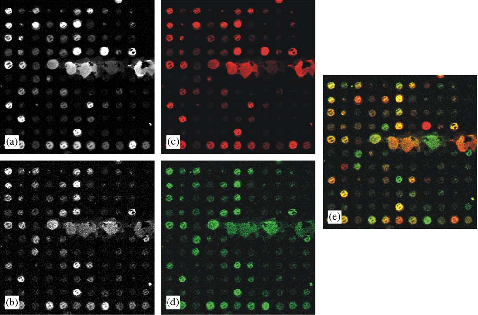
\includegraphics[width=0.8\textwidth]{img/intro/2_meth_transcripto/intro_2_true_microarray_picture_10.1016_j.fss.2004.10.012.png}
    \caption[Image d'une puce à ADN à deux canaux rouge et vert]{Image d'une puce à ADN à deux canaux rouge et vert. (a) Canal rouge en échelle de gris, (b) Canal vert en échelle de gris, (c,d) Canaux respectifs colorés selon leur fluorescence, (e) Puce à ADN visualisée en coloration RGB (\textit{Red Green Blue}). Des artefacts de fluorescence sont visibles en ligne 5. Issu de Lukac \textit{et al.} 2005 \cite{Lukac2005May}.}
    \label{fig:intro_true_microarray_picture}
\end{figure}

L'intensité de fluorescence, aussi appelée abondance, détectée par le capteur constitue la donnée retournée pour un transcrit donné sur une puce à ADN en théorie. Comme on peut le voir en Figure \ref{fig:intro_true_microarray_picture}, cette abondance n'est toutefois pas uniforme au sein d'un même puits. L'image capturée va donc rarement être utilisée en tant que telle pour donner les abondances chiffrées finales et va passer par un premier ensemble d'ajustements.

En 2004, Petrov \textit{et al.} \cite{Petrov2004Nov} ont ainsi exploré en détail l'impact de différents paramètres expérimentaux et de différents choix de correction du signal en se basant sur un contrôle qualité approfondit des puces étudiées. Le pré-traitement de l'image prise d'une puce à ADN y est découpé selon 4 étapes, plus une s'il s'agît d'une puce à deux canaux : l'alignement d'images si deux canaux, le placement de grille, la détection de puits, la segmentation et la mesure de qualité (Figure \ref{fig:intro_microarray_image_preprocessing}). Ces étapes permettent en finalité d'assurer la reproductibilité de la valeur d'abondance détectée, ainsi qu'une robustesse face à des évènements tels que des artefacts de fluorescences, des contaminations de puits, ou encore des variations de fluorescence entre réplicats.

\begin{figure}[b]
    \centering
    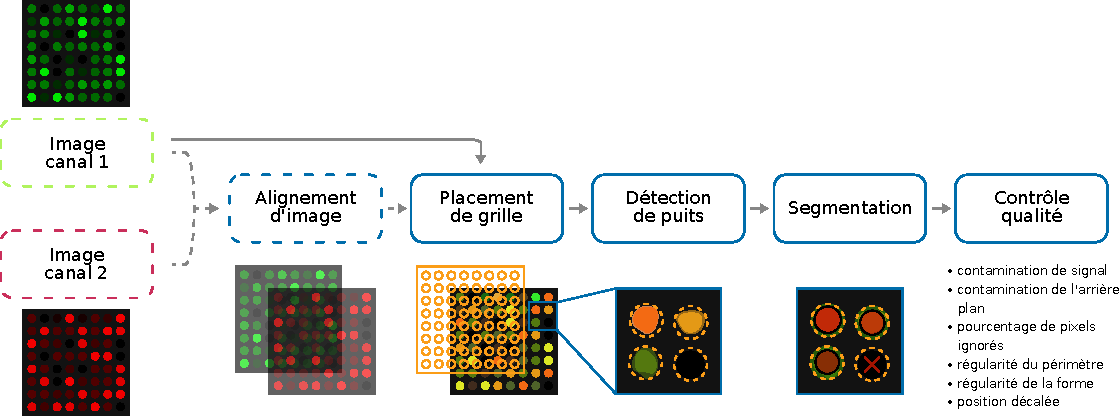
\includegraphics[width=\textwidth]{img/intro/2_meth_transcripto/intro_2_microarray_image_preprocessing.pdf}
    \caption[Ordre des différentes étapes de pré-traitement d'une image de puce à ADN]{Ordre des différentes étapes de pré-traitement d'une image de puce à ADN. Modifié d'après Petrov et al \cite{Petrov2004Nov}.}
    \label{fig:intro_microarray_image_preprocessing}
\end{figure}

Une fois cette étape de traitement de l'image effectuée, de nombreux biais techniques peuvent encore impacter la valeur chiffrée retournée depuis l'image corrigée. On applique donc une étape dite de normalisation qui visera tant à palier les biais techniques contrôlables qu'incontrôlables afin de comparer au mieux différentes conditions. Bien que la variété de modèles de puces à ADN et de conditions d'utilisation puisse nécessiter l'utilisation de normalisations spécifiques, trois approches font consensus \cite{Smyth2003Dec} (Figure \ref{fig:intro_microarray_normalization}) : la normalisation d'arrière-plan, la normalisation intra-puce, et la normalisation inter-puces.

% Si des normalisations consensus existent, la variété de modèles de puces à ADN et de conditions d'utilisation peut demander l'utilisation de normalisations supplémentaires. On se concentrera ici sur les normalisations consensus uniquement \cite{Smyth2003Dec} (Figure \ref{fig:intro_microarray_normalization}) bien qu'on mentionnera brièvement d'autres normalisations plus contextuelles. 

\begin{figure}[b]
    \centering
    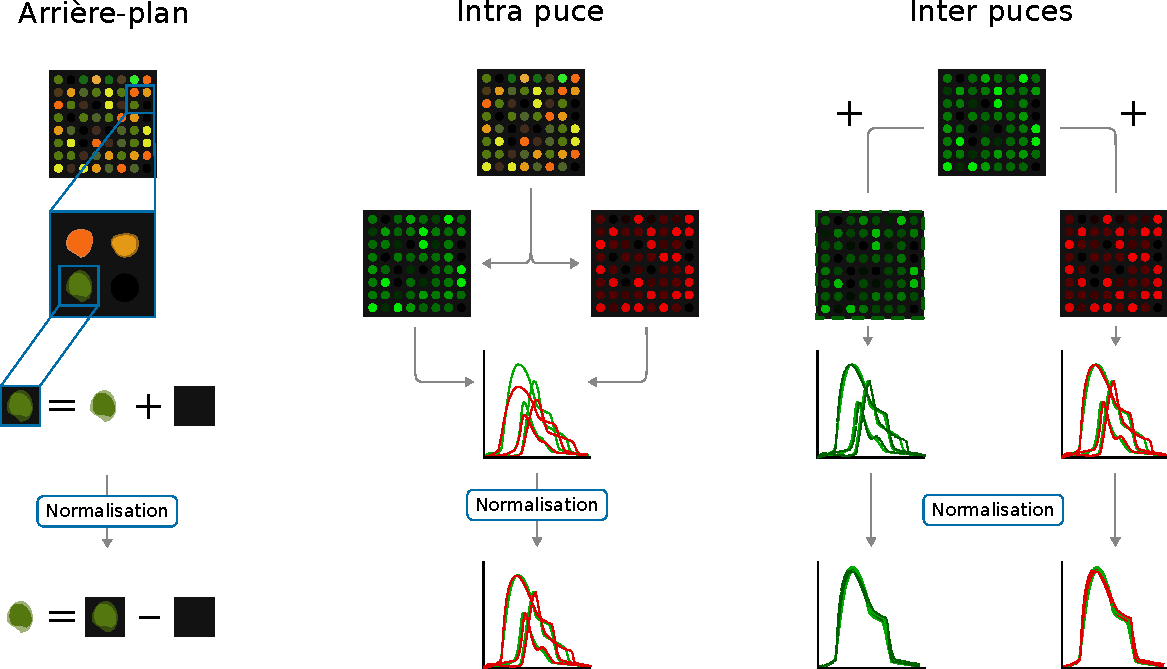
\includegraphics[width=\textwidth]{img/intro/2_meth_transcripto/intro_2_microarray_normalization.pdf}
    \caption[Normalisations consensus de puces à ADN]{Normalisations consensus de puces à ADN : la normalisation de l'arrière-plan, la normalisation intra puce, et la normalisation inter puces.}
    \label{fig:intro_microarray_normalization}
\end{figure}

La normalisation de l'arrière-plan va venir corriger le biais d'intensité parasite lié au phénomène d'hybridation non spécifique des transcrits sur les amorces dans les puits. Par une simple soustraction de l'intensité de l'arrière-plan à l'intensité détectée dans chaque puits on va permettre de compenser le biais. Lors de l'utilisation d'une puce à deux canaux, les intensités en fonction de la fluorescence utilisée tendent à ne pas couvrir le même intervalle d'intensité. Il est possible également que d'autres biais non-linéaires impactent les différents canaux de la puce. Ces biais sont corrigés par une normalisation dite intra-puce et n'est donc généralement pas utilisée dans le cas de puce à un canal. Plusieurs méthodes se sont succédé pour réaliser cette normalisation avec dans les débuts une utilisation d'un puits de contrôle, de la somme de toutes les intensités, ou de la déviation absolue médiane pour diviser les intensités de chaque transcrit. Plus récemment, l'approximation des données par une régression pondérée locale (en anglais \textit{LOESS} pour \textit{LOcally Estimated Scatterplot Smoothing}) inspirée du théorème de Taylor et aboutie par Cleveland et Devlin en 1988 \cite{Cleveland1988Sep} a prouvé être particulièrement efficace pour retirer ce biais intra-puce \cite{Smyth2003Dec}. Enfin, la finalité des puces à ADN dans l'analyse d'expression de gène étant la comparaison de \glspl{condition}, on va effectuer une étape de normalisation inter-puces pour s'assurer de leur comparabilité pour détecter au mieux les variations significatives entre elles. Cette correction consiste donc à rendre similaire la distribution des intensités. La méthode variera cependant selon le type et le nombre de canaux des puces bien que la plupart soient une adaptation d'une normalisation par quantiles \cite{Ritchie2015Apr}. \\


À ces normalisation s'ajoutent d'autres transformations usuelles des données des puces à ADN telles que des filtrations \cite{Quackenbush2002Dec}. On y retrouve la suppression des données d'intensité des transcrits dont la fluorescence du puits aurait saturé le capteur et engendré une quantification tronquée \cite{Wilkes2007Apr}. Lors de l'utilisation de réplicats biologiques, les transcrits présentant une faible intensité après normalisation de l'arrière-plan et une faible variation entre les réplicats peuvent être supprimées des données. Également, il est d'usage de transformer les données d'intensité en logarithme, le plus souvent un log2. Ce changement d'une expression en échelle additive en une échelle proportionnelle de facteur 2 vise à faciliter l'interprétation. En effet, dans cette disposition, une intensité augmentant ou diminuant de 1 unité signifiera respectivement un doublement ou une division par deux de l'intensité \cite{Smyth2003Dec}, ce qui est souvent considéré comme un changement de l'expression significatif en biologie. 

Ces différentes normalisations et transformations peuvent mathématiquement se réaliser dans n'importe quel ordre. Toutefois, bio-informatiquement, il est important de s'attacher à l'ordre et au choix des méthodes employées car chacune possède des contraintes, un contexte d'utilisation, et doit tenir compte du type d'analyse réalisée sur les données par la suite. On parle alors de stratégie de normalisation. Parmi les précautions à prendre dans la stratégie, il est par exemple nécessaire lors d'analyses comparatives de conditions de tenir compte des transcrits supprimés d'une des deux puces à ADN uniquement. Dans le cas contraire, une différence significative artificielle pourrait être obtenue, faussant alors les résultats. De même, l'étape de normalisation intra-puce doit être faite avec parcimonie car elle peut entraîner dans certains cas une non-comparabilité ultérieure avec d'autres puces en fixant la distribution relativement à la puce considérée \cite{Argyropoulos2006Apr}. Enfin, plus généralement, une utilisation à mauvais escient de certaines normalisations peut aussi entraîner une suppression du signal biologique d'intérêt. Une fois totalement préparées, ces données peuvent finalement être analysées par diverses méthodes pour détecter des différences d'expression.

% Le package R \textit{limma} hébergé sur le dépôt Bioconductor \cite{Gentleman2004Sep} regroupe l'intégralité de ces normalisations de même que d'autres outils de contrôle qualité et est ainsi devenu une référence dans la normalisation post traitement d'image et plus généralement l'analyse de puces à ADN.


Mais face à la limitation en nombre de transcrits et à l'impossibilité de quantifier des transcrits inconnus, l'utilisation de puces à ADN tend à diminuer de plus en plus au profit du RNA-seq. Bolon-Canedo \textit{et al.} soulignent ainsi en 2019 \cite{Bolon-Canedo2019} qu'elles ne sont plus pertinentes à ce jour pour de la recherche exploratoire telle que l'étude du transcriptome de nouveaux organismes ou l'analyse comparative de l'expression dans des conditions mal comprises.
L'utilisation des puces à ADN reste toutefois pertinente dans d'autres types d'analyses plus ciblées de transcrits. Elles restent un outil au rapport qualité/prix imbattable dans des analyses de génotypage pour du diagnostic ou de l'étude de population.


%% Sources d'aide à la rédaction
% Un TRES bon site sur les technos de sequencage : http://education.knoweng.org/sequenceng/

%% Infos potentiellement rajoutables :
% RAjouter une explication d'en quoi consiste chaque étape ?

%% INFOS ET FORMULATION SUR LA NORMALISATION
% Parmi les biais biologiques classiques, on retrouve le contenu en GC, la longueur des transcrits, la quantité d'ARN total,  weighted linear regression (lowess).
% Pour corriger ces biais biologiques, plusieurs méthodes ont été proposées prenant chacune plus ou moins de biais en compte  : 
% linear regression analysis1, log cen- tering, rank invariant methods2 and Chen’s ratio statistics3
% SOURCE : 10.1038/ng1032


\subsection{RNA-Seq}

\subsubsection{Principe}

Aujourd'hui, le séquençage de l'ARN (RNA-seq) est devenu la technologie privilégiée pour les études \glspl{transcriptomique}. Issue des techniques de séquençage nouvelle génération, le RNA-seq permet d'étudier le \gls{transcriptome} d'un \gls{organisme} sans connaissance préalable de sa séquence \cite{Wang2009Jan}. Le protocole de préparation des transcrits est le même que pour les puces à ADN sauf dans le cas d'un séquençage direct de l'ARN. Après prélèvement des échantillons, les transcrits sont isolés par purification et rétro-transcrits en ADNc. Ceux-ci sont alors amplifiés par PCR et fragmentés selon la taille requise par la technologie de séquençage. Le séquençage peut se faire actuellement par seconde ou troisième génération dépendant de l'objectif poursuivit. Les technologies de seconde génération, avec notamment celle d'Illumina (Figure \ref{fig:intro_rnaseq_workflow}), sont ainsi adaptées dans le cadre d'une comparaison de \glspl{condition}. Elles produisent rapidement un séquençage au rapport qualité prix raisonnable avec un minimum de 30 millions de lectures (en anglais \textit{reads}) alignées recommandées par le projet ENCODE \cite{ENCODE2012} pour de l'ARN total chez l'humain. Les technologies de troisième génération telles que PacBio ou Nanopore (Figure \ref{fig:intro_rnaseq_workflow}) quant à elles prennent plus de temps mais peuvent séquencer des fragments de taille bien supérieure à ceux de seconde génération. Cette capacité les rend donc particulièrement adaptées à l'analyse de la variété de transcrits issus de l'épissage alternatif \cite{Bergsma2018Jan}. 

\begin{figure}[hb]
    \centering
    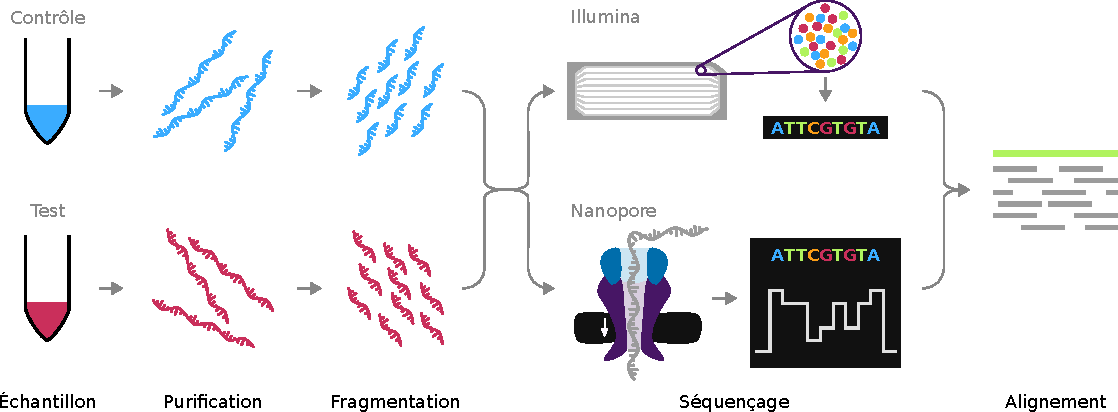
\includegraphics[width=\textwidth]{img/intro/2_meth_transcripto/intro_2_rnaseq_workflpow.pdf}
    \caption{Déroulé d'une opération de quantification d'expression par RNA-seq.}
    \label{fig:intro_rnaseq_workflow}
\end{figure}

Les lectures de ces fragments sont ensuite alignées sur un transcriptome de référence ou bien sont l'objet d'un assemblage de transcriptome \textit{de novo}, c’est-à-dire un nouvel assemblage sans connaissance préalable. Plusieurs méthodes partant de différents postulats existent pour réaliser cette étape d'alignement loin d'être triviale. Chacune possède ses avantages et limites qu'il faut toutefois prendre en compte en cela qu'elles impactent l'expression finale quantifiée \cite{Yi2018Oct,Srivastava2020Dec}. Dans la catégorie des associations aligneurs et quantifieurs utilisés pour la quantification, les aligneurs STAR \cite{Dobin2013Jan} et minimap2 \cite{Li2018Sep} associés au quantifieur RSEM \cite{Li2011Dec} sont parmi les plus utilisés et donnent des quantifications extrêmement précises car ils donnent la position de chaque lecture de transcrits sur un génome de référence ou \textit{de novo}. Ces aligneurs sont cependant assez lents et notamment dans le cas d'un alignement \textit{de novo}. À l'opposé se trouvent les logiciels Salmon \cite{Patro2017Apr} et Kallisto \cite{Bray2016May}, des quantifieurs basés sur un principe de d'alignement probabiliste nommé \textit{selective-alignment} pour Salmon et \textit{pseudo-alignment} pour Kallisto. Plus rapides que les aligneurs classiques, ils sont, en raison de leurs euristiques, plus sujets aux erreurs de quantification bien qu'elles restent rares. Ces aligneurs probabilistes sont également incapables de détecter de nouveaux gènes étant donné leur utilisation d'un index de transcriptome. Quelle que soit la méthode employée pour comptabiliser les lectures par transcrit, ces données doivent ensuite être traitées avant d'être analysées.



\subsubsection{Pré-traitement des données}

Comme les puces à ADN, le RNA-seq nécessite de normaliser et transformer les données pour les rendre exploitables en retirant les biais techniques et biologiques. Des contrôles qualité existent ainsi pour contrôler dans un premier temps d'éventuels artefacts de séquençage tels que la sur-représentation d'une lecture, ou encore des erreurs de formatage ou d'encodage des fichiers par exemple. Concernant la normalisation, une des approches est la division des comptes bruts par la profondeur de séquençage et 1 million, ce qui donne des comptes par million (en anglais \textit{count per million} ou CPM). Si cette normalisation est assez courante comme d'autres normalisations, elles ne peuvent toutefois être appliquées de façon systématique. La normalisation donnant des fragments par million de kilobases (en anglais \textit{Fragments Per Kilobase Million} ou FPKM) pour le séquençage à lecture par paire (en anglais \textit{paired-end}) ou des lectures par million de kilobases (en anglais \textit{Fragments Per Kilobase Million} ou RPKM) lorsqu'il s'agit de séquençage à lecture unique (en anglais \textit{single-end}) sont ainsi des normalisations à éviter lors d'analyses comparatives \cite{Wagner2012Dec}. En divisant directement les CPM par la longueur des gènes pour tenir compte du biais de comptage en faveur des gènes de plus grande taille, l'utilisation de la normalisation en FPKM/RPKM entraîne potentiellement une somme de lectures normalisée différente dans chaque échantillon. L'analyse comparative étant un des intérêts majeur de la \gls{transcriptomique} en recherche, en médecine moléculaire et en biologie, d'autres mesures normalisées compatibles avec ce type de problématique ont été développées. Le RLE, pour \textit{Relative Log Expression} \cite{Anders2010Oct} et le TMM pour \textit{Trimmed Mean of M-values} \cite{Robinson2010Mar} sont ainsi des normalisations recommandées par l'étude du French StatOmique Consortium\footnote{Dans cette publication, le RLE est introduit par le biais du progiciel (en anglais \textit{package}) DESeq \cite{Anders2010Oct} qui implémente cette mesure} en 2013 \cite{Dillies2013Nov}. Tous deux partent du principe que l'expression de la majorité des gènes ne change pas entre deux \glspl{condition}. Le RLE consiste tout d'abord à calculer une pseudo référence (Équation \ref{pseudoref}) via une moyenne géométrique sur tous les échantillons \cite{Gandolfo2018Feb} qui contrairement au RPKM conserve bien une somme de lectures identique entre échantillons et est moins sensible aux valeurs extrêmes que la moyenne arithmétique. Un facteur de taille (Équation \ref{sizefactor}) est ensuite calculé comme la médiane des rapports entre les comptages de chaque échantillon avec ceux de la pseudo-référence. Celui-ci est alors utilisé pour normaliser les comptes bruts de chaque échantillon.
% Celui-ci est alors utilisé pour calculer les paramètres $\mu_{i j}$ et $\sigma^2_{i j}$ de la loi binomiale négative qui sert à estimer les comptes de lectures d'un échantillon $j$ pour un gène $i$ (Équation \ref{readcount}).

\begin{equation}\label{pseudoref}
    \text{pseudo-référence} = \left(\prod_{t=1}^{m} k_{i t}\right)^{1 / m}
\end{equation}

\begin{equation}\label{sizefactor}
    \text{facteur de taille} = \hat{s}_{j}=\underset{i}{\operatorname{median}} \frac{k_{i j}}{\left(\prod_{v=t}^{m} k_{i t}\right)^{1 / m}}
\end{equation}

% \begin{equation}\label{readcount}
%     \text{comptes de lectures} = K_{i j} \sim NB(\mu_{i j}, \sigma^2_{i j})
% \end{equation}

Où :
\begin{align*}
i & = \text{gène} = 1,..., n \\
j & = \text{échantillon} = 1,..., m \\
k & = \text{table de comptes de lectures observés } n \times m 
\end{align*}

Le TMM quant à lui effectue une normalisation par le nombre de fragments d'ARN pour chaque gène dans chaque échantillon et s'en sert pour calculer la valeur M qui est rapport du niveau moyen en base 2, soit un log2 entre les échantillons de deux conditions (Équation \ref{mvalue}). Certains comptes pouvant être nuls ce que ne peut accepter un logarithme, il est d'usage d'employer des pseudo-comptes qui sont des comptes auxquels on a ajouté 1 \cite{Booeshaghi2021Mar}. Parallèlement, il calcule la valeur A qui est la valeur absolue du niveau d'expression (Équation \ref{avalue}). Ces deux valeurs sont respectivement tronquées de 30\% et 5\% et servent à estimer une moyenne pondérée d'après un échantillon référence qui est l'échantillon au 3\textsuperscript{ème} quartile le plus proche de la moyenne des 3\textsuperscript{èmes} quartiles (Équation \ref{weightedmean}) qui permet enfin de calculer le facteur de normalisation (Équation \ref{normtmmfactor}).

\begin{equation}\label{mvalue}
    M_g = \log_{2} \left(\frac{Y_{gk} / N_k}{Y_{gk'} / N_k'}\right)
\end{equation}

\begin{equation}\label{avalue}
    A_g = \frac{1}{2} \left(\log_{2} \left(\frac{Y_{gk}}{N_k} \right) + \log_2 \left(\frac{Y_{gk'}}{N_k'}\right)\right)
\end{equation}

\begin{equation}\label{weightedmean}
    w^r_{gk} = \frac{N_k - Y_{gk}}{N_k \times Y_{gk}} + \frac{N_r - Y_{gr}}{N_r \times Y_{gr}}
\end{equation}

\begin{equation}\label{normtmmfactor}
    \log_2{} (TMM^r_k) = \frac{\sum_{g \in G^*} w^r_{gk} \times M^r_{gk}}{\sum_{g \in G^*} w^r_{gk}}
\end{equation}

Où :
\begin{align*}
    g & = \text{gène} \\
    k & = \text{échantillon} \\
    N_{\dots} & = \text{nombre total de lectures pour \dots (soit }k \text{, soit r)} \\
    Y_{g\dots} & = \text{comptes observés pour \dots (soit }k \text{, soit r)} \\
    r & = \text{référence} \\
    G^* & = \text{ensemble des gènes non tronqués lors du tronquage de } M_g \text{ et } A_g
\end{align*}

% Now, double trim the upper and lower percentages of the data (trim M values by 30% and A values by 5%)
% Get weighted mean of M after trimming and calculate normalization factor 

Une étude détaillée des performances et propriétés mathématiques du RLE et du TMM a par ailleurs été publiée en 2016 en reprenant les différentes étapes de leur normalisation pour en tirer des équivalences \cite{Maza2016} (Figure \ref{fig:maza2016_table2}). À ces méthodes de normalisation s'en ajoutent d'autres se basant sur le contenu en GC qui va favoriser le séquençage de gènes par rapport à d'autres \cite{Filloux2014Dec}. D'autres méthodes encore utilisent des gènes contrôle, le plus souvent des gènes dit de ménage (en anglais \textit{housekeeping genes}) \cite{Zhou2017Sep} à l'instar des puces à ADN. Chaque méthode de normalisation va donc modifier considérablement la distribution des données d'expression et la stratégie de normalisation mise en place va et doit donc dépendre de l'analyse ultérieure faite sur les données. 
% Dans le cadre de cette thèse qui aborde l'analyse par réseaux de co-expression de gènes, on ne considèrera par exemple qu


\begin{figure}[hb]
    \centering
    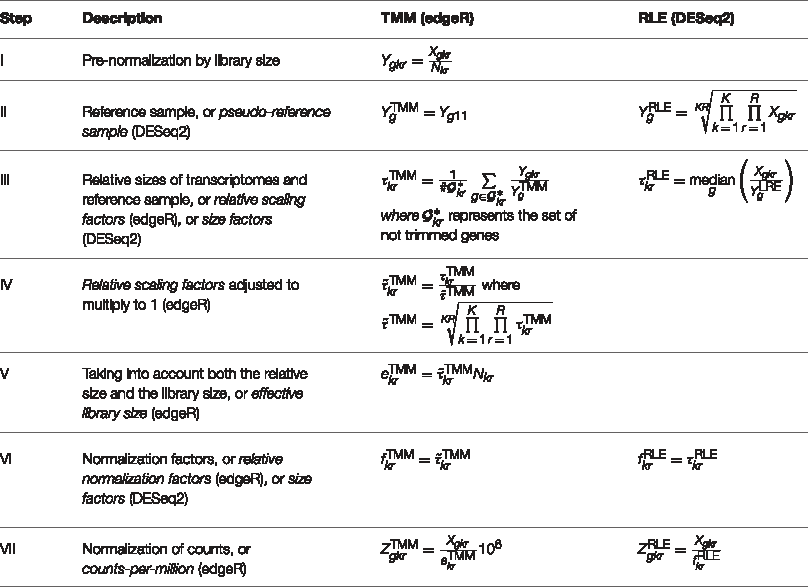
\includegraphics{img/intro/2_meth_transcripto/intro_2_maza2016_table2.pdf}
    \caption[Table de comparaison des étapes de normalisation avec équivalences re-exprimées]{Table de comparaison des étapes de normalisation avec équivalences re-exprimées. Issu de la Table 2 (tronquée) de Maza 2016 \cite{Maza2016}.}
    \label{fig:maza2016_table2}
\end{figure}


% Aide sur les méthodes et unités de normalisation : https://www.reneshbedre.com/blog/expression_units.html


\section{L'analyse transcriptomique par réseaux de co-expression}

L'explosion de la taille et quantité de jeux de données mis à disposition publiquement engendre une demande croissante en techniques d'analyse capable de les gérer mais également de profiter de la précision de séquençage apportée. L'analyse d'expression différentielle fut la première méthode dédiée spécifiquement à l'analyse des données de quantification d'expression contrairement à des méthodes de statistique exploratoire comme l'analyse par composantes principales (ACP) \cite{deKok2005Jan}. Elle consiste à comparer l'expression de chaque gène entre différentes \glspl{condition}, le plus souvent un contrôle contre un test, pour déterminer avec un test statistique quels gènes voient leur expression significativement changer dans la condition test. Si plusieurs méthodes ont été développées pour s'assurer de la robustesse de l'identification des gènes différentiellement exprimés \cite{Soneson2013Dec,Spies2019Jan}, le principe reste le même : identifier les gènes sur-exprimés ou sous-exprimés. Dans la recherche permanente qu'est la priorisation de gènes candidats à une maladie, l'analyse d'expression différentielle a donc grandement contribué à l'approfondissement de la connaissance de certaines pathologies et a permis d'y associer des biomarqueurs pour réaliser des diagnostics \cite{Costa-Silva2017Dec}. Outre les problèmes de reproductibilité soulevés par plusieurs études \cite{Ostlund2014}, les analyses d'expression différentielle présentent 
également l'inconvénient d'être limitées à quelques gènes d'un ou plusieurs \glspl{mecanisme} qui impliquent pourtant bien plus de gènes. À titre d'exemple, nombre de gènes associés à des maladies Mendéliennes sont exprimés dans plusieurs tissus sans entraîner nécessairement de dysfonctionnement, suggérant plutôt une interaction délétaire qu'un gène problématique à lui seul \cite{Hekselman2020Mar}. De plus, l'analyse d'expression différentielle est mise en difficulté dans le cas de gènes à large variance à travers les échantillons étant donné la tendance des plages de valeurs d'expression à se chevaucher \cite{Ostlund2014}. Elle en vient alors à manquer de sensibilité et va omettre des gènes dont l'implication est effective dans certaines condition \cite{delaFuente2010Jul}. L'analyse par réseaux de co-expression de gènes a notamment été développée dans l'optique de répondre à ce type de problématique. En ne considérant non pas seulement les gènes mais leur dynamique ou profil d'expression et leur synchronisation, les réseaux de co-expression visent à identifier les motifs de variation de la transcription qui indiquent des interactions fonctionnelles ou de régulation des relations entre gènes \cite{Parsana2019}. La découverte d'information est cependant rarement faite à partir du simple réseau construit. Pour discerner les gènes interagissant préférentiellement ensemble, une méthode de partitionnement est appliquée et va définir des groupes de gènes qu'on nomme \glspl{module}. Ceux-ci sont ensuite interprétés à l'aide de différentes méthodes incluant de la connaissance a priori, ou de l'analyse topologique pour de la connaissance \textit{ex nihilo}. Il en résulte un pipeline d'analyse (Figure \ref{fig:coexpr_pipeline}) \cite{Zhang2005a} qu'on va décrire en détail dans les parties qui suivent.


\begin{figure}[ht]
    \centering
    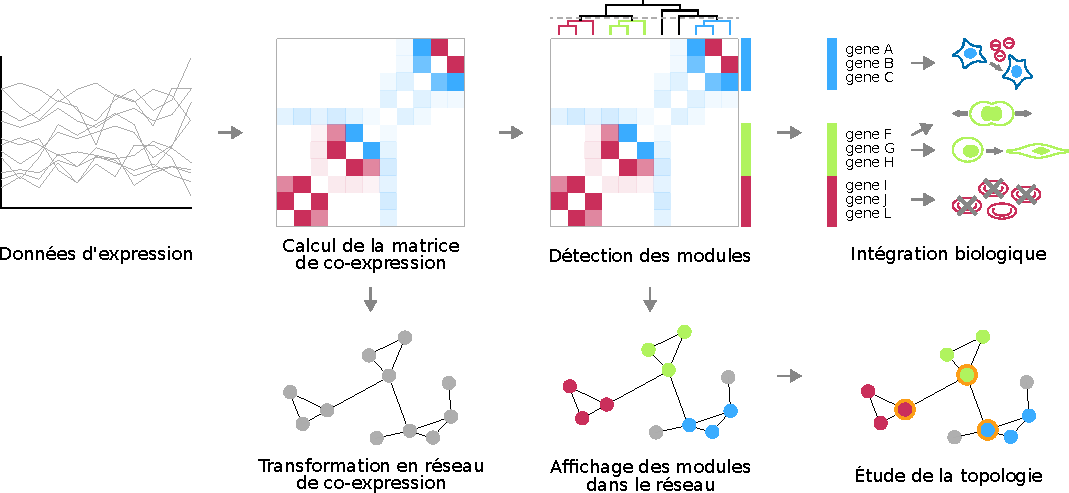
\includegraphics[width=\textwidth]{img/intro/3_coexpr/intro_3_coexpr_principle.pdf}
    \caption[Étapes de réalisation d'une analyse par réseaux de co-expression.]{Étapes de réalisation d'une analyse par réseaux de co-expression.}
    \label{fig:coexpr_pipeline}
\end{figure}



% \subsection{Principe de la co-expression et définitions des réseaux}
\subsection{Définitions des réseaux et principe de la co-expression}

L'analyse par réseaux de co-expression de gènes (en anglais \acrfull{GCN}) a su bénéficier des avancées conceptuelles en théorie des réseaux depuis sa conception pour encoder et étudier au mieux les relations entre gènes \cite{Barabasi2011Jan}. La théorie des réseaux appartient elle-même à la théorie des graphes, structure mathématique derrière les réseaux \cite{Barnes1983Jun}. Un \textbf{\gls{reseau}} n'est en effet qu'une implémentation d'un \textbf{\gls{graphe}}, un cas particulier, pour représenter des entités et leur connections dans un contexte donné. Ainsi, si les termes de graphe et réseau sont souvent utilisés de façon interchangeable hors de la recherche en informatique et mathématique, il est à noter qu'ils désignent des concepts différents bien qu'imbriqués, et au vocabulaire spécifique. Ainsi, les entités considérées, ici les gènes, sont appelés \textbf{nœuds} dans un réseau et \textbf{sommets} dans un graphe. De même, les connections reliant les entités seront nommées respectivement \textbf{lien} et \textbf{arrête}. Dans cette thèse, les termes de nœud et lien seront donc préférés car issus de la théorie des réseaux. Les liens représentent de façon binaire la présence (valeur du lien égale à 1) ou l'absence, (valeur égale à 0) de relation entre les nœuds. Les relations entre gènes en biologie ne sont toutefois pas aussi dichotomiques et nécessitent plus de granularité pour décrire la multiplicité et le niveau des interactions. Une même cellule échantillonnée à des temps différents aura un profil plus ou moins différent où les fonctions clefs auront peu changé mais celles plus variables auront varié bien plus. C'est pourquoi on utilise plus souvent des réseaux dit pondérés qui vont ajouter une valeur réelle $\mathbb{R}$, le plus souvent décimale $\mathbb{D}$ entre 0 et 1 qui vont représenter une force de liaison entre deux gènes. Si le réseau est \textbf{signé}, ces valeurs seront en plus positives si le lien représente une co-expression conjointe, et négative s’il représente une co-expression opposée (Figure \ref{fig:coexpr_corr_weight_sign}).

\begin{figure}[ht]
    \centering
    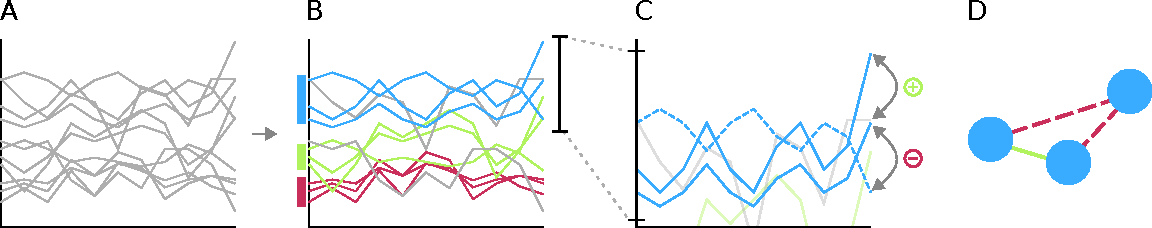
\includegraphics[width=\textwidth]{img/intro/3_coexpr/intro_3_coexpr_expr_group_sign.pdf}
    \caption[Définition des liens du réseau pour des gènes se co-exprimant.]{Définition des liens du réseau pour des gènes se co-exprimant. A. Profils d'\gls{genexpr} selon plusieurs échantillons avec en bleu 3 gènes co-exprimés. B. Zoom sur l'expression de ces 3 gènes avec mise en avant de deux gènes avec un profil dans un sens et un gène avec un profil dans le sens inverse; les deux profils en sens identique ont donc un score de similarité positif entre eux, et négatif avec le troisième gène. C. Ces scores et leur signe sont utilisés pour visualiser les liens entre ces gènes sous forme de nœuds dans un réseau.}
    \label{fig:coexpr_corr_weight_sign}
\end{figure}

Lorsque deux nœuds sont reliés par un lien, on dit qu'ils sont \textbf{\glspl{voisin}}. De cette unité de base vont découler plusieurs mesures qui vont permettre de caractériser un réseau du point de vue de sa topologie. Le \textbf{\gls{degre}} d'un nœud est ainsi le nombre de voisins dont il dispose tandis que la somme des valeurs des liens pondérés ou non sera appelée la \textbf{force} ou la \textbf{connectivite} d'un nœud selon le contexte. À l'échelle du réseau on va retrouver des mesures qui vont permettre de localiser des zones aux propriétés différentes du reste du réseau. Le cumul des \textbf{\gls{plus_court_chemin}} pour se rendre d'un nœud à un autre est ainsi un moyen de mesurer la \textbf{centralité} d'une zone ou d'un nœud. Ces métriques peuvent également tenir compte de la direction des liens si une direction est précisée. Dans ce cas on parle de réseau dirigé en opposition avec les réseaux non dirigés où le sens du lien est inconnu ou inexistant. Habituellement cependant, les \acrshort{GCN} sont non dirigés car leur construction ne permet pas nativement de déterminer une causalité. 

Les \acrshort{GCN} se construisent conventionnellement à partir d'une matrice d'expression $n \times m$ d'indice $i = 1 \dots n$ pour les échantillons et de variable $j = 1 \dots m$. Une métrique est alors calculée sur chaque paire de gènes pour quantifier leur relation. Plusieurs approches existent dans le choix d'une métrique comme des modèles de mélange gaussien ou des probabilités bayésiennes. Mais l'approche la plus commune et sur laquelle on s'est concentré durant cette thèse est une approche par score de similarité. Ce terme généraliste permet d'englober la quantité importante de méthodes employée pour quantifier la similarité des gènes deux à deux. 



\subsection{Considérations préalables à l'analyse par réseaux de co-expression de gènes}

% De même qu'il a fallut normal
L'analyse de données d'\gls{genexpr} par réseaux de co-expression nécessite des précautions et préparations en plus de celles effectuée sur chaque technologie de \gls{transcriptomique}. Sur le plan de la normalisation, certaines normalisations de puce à ADN et de RNA-seq ne seront pas compatible avec l'analyse par co-expression telle que décrite dans la section suivante \cite{Zhang2005a}. Pour des données provenant de RNA-seq, les normalisations FPKM/RPKM et TPM ou tout autre normalisation visant à corriger pour le nombre total de lectures ou la taille des gènes sont à proscrire. En présence de gènes très fortement exprimés, le restant des gènes va décroître relativement ce qui va entraîner une co-expression artificielle entre ces gènes \cite{Spiko2017thesis}. Les informations pointant vers une normalisation adaptée en particulier pour le RNA-seq en co-expression sont toutefois manquantes\footnote{À ce jour et lors de la réalisation des travaux présentés dans cette thèse. Une publication préliminaire (en anglais \textit{preprint}) réalisé par A. Vandenbon en mars 2021 \cite{Vandenbon2021Mar} a toutefois réalisé une comparaison étendue de 6 normalisations pour relever que le quartile supérieur est la méthode la plus adaptée globalement.}. Les TMM et RLE sont conceptuellement compatibles mais les dernières publications tendent à utiliser la correction par composante principale \cite{Parsana2019} qui effectue en plus une correction de multiples biais et va retirer des facteurs confondants non identifiés. Ces facteurs confondants sont d'ailleurs une source majeure de co-expression erronée car ils favorisent la corrélation de gènes sur des critères indépendants de la question biologique étudiée. Dans le cas des puces à ADN, une étude de Reverter \textit{et al.} trouve la normalisation par modèles mixtes comme idéale \cite{Reverter2005Apr}. Cependant, une étude de Lim \textit{et al.} trouve plus tard le MAS5 comme idéal mais sans comparaison avec la normalisation par modèle mixte \cite{Lim2007Jul}.

Malgré une normalisation visant à donner des résultats les plus proches de la vérité possible, chacune des technologies de transcriptomique, même si effectuées sur des échantillons identiques, va donner des réseaux différents comme l'a étudié Giorgi \textit{et al.} \cite{Giorgi2013Mar}. Les réseaux basés sur des puces à ADN tendant à être plus similaires aux réseaux biologiques déjà connus par rapport au RNA-seq. Un biais est toutefois présent dans cette conclusion car les réseaux biologiques en question influent en partie le design des puces à ADN en termes de transcrits mesurés. Ainsi, les réseaux basés sur RNA-seq sont moins similaires aux réseaux biologiques car ils prennent en compte la totalité des transcrits présents et permettent une meilleure découverte de nouveaux gènes d'intérêt. La nature de cette différence, signal réel ou bruit, est toutefois un cas particulier à chaque couple réseau/\gls{organisme}. Ballouz \textit{et al.} sont venu en 2015 \cite{Ballouz2015} préciser les différences et ont constaté que la différence majeure repose sur la variation de topologie et plus particulièrement de connectivité. De nombreux gènes détectés comme pivot dans les réseaux basé sur puce à ADN ne sont pas retrouvés dans ceux à RNA-seq et inversement bien que leurs propriétés fonctionnelles soient les mêmes. En investiguant la contribution des transcrits aux gènes pivots, ils concluent que le RNA-seq tend à capturer plus de variation d'expression dans les données, mais qu'il est en contrepartie très sensible au bruit causé par les faibles intensités d'expression. 

Le nombre d'échantillons disponibles pour construire le \acrshort{GCN} va également impacter sa topologie finale et les informations pouvant en être extraites. Plus il a d'échantillons, plus la qualité des \acrshort{GCN} tend à s'améliorer, cependant cette relation que Ballouz et al définissait comme linéaire, ne l'est pas. Liesecke \textit{et al.} ont démontré en 2019 que celle-ci atteint un plateau qui dépend de la technologie de transcriptomique \cite{Liesecke2019}. À taille d'échantillons équivalente, les réseaux de puces à ADN permettent une meilleure découverte de fonctions physiologiques. Ceci est toujours à mettre en perspective avec le fait que le RNA-seq comprends plus de transcrits et que de nombreuses fonctions physiologiques sont issues d'analyses sur puce à ADN, et que d'autres fonctions sont encore à découvrir avec l'avènement du RNA-seq. En finalité, il est recommandé d'utiliser au minimum 100 échantillons pour la construction d'un réseau, bien qu'un nombre inférieur soit utilisable à la condition d'assurer une qualité des données via une normalisation et correction des artéfacts rigoureuse. 

Tous les transcrits ne sont également pas bon à prendre en compte dans une construction de \acrshort{GCN}. Leur filtration cependant doit tenir compte des propriétés et postulats faits par les méthodes de construction du \acrshort{GCN}, car une filtration mal menée peu significativement altérer le réseau. Une erreur courante est ainsi de n'utiliser que les gènes différentiellement exprimés pour construire un réseau, ce qui va changer la loi de distribution de l'expression sur laquelle de nombreuses méthodes se basent \cite{Zhang2005a}. À l'inverse, certaines filtrations vont être essentielles afin de réduire le bruit dans l'expression. Les gènes ayant une très faible variation d'expression entre échantillons sont ainsi à retirer des jeux de données car ils vont avoir tendance à corréler entre eux. De même en RNA-seq, on retirera les gènes dont le nombre de lectures est inférieur à un seuil dépendant du séquenceur. Similairement dans les puces à ADN, on supprimera les gènes dont les intensités sont proches du seuil minimal de détection. En considérant l'intégralité de ces précautions avant la construction d'un \acrshort{GCN}, il est possible d'assurer un réseau représentatif de la condition étudiée.



\subsection{Construction}

\subsubsection{Score de base}

La méthode de construction abordée dans cette thèse se focalise sur une approche par score de similarité entre gènes deux à deux. Si ce score était initialement basé sur une approche naïve par corrélation de Pearson \cite{Carter2004} (Équation \ref{simscore_base_pearson}), d'autres scores plus robustes ont depuis été proposés. Ainsi, La corrélation de Spearman (Équation \ref{simscore_base_spearman}) est une méthode couramment utilisée en raison de sa faible sensibilité aux artefacts grâce à sa corrélation par rang \cite{Chowdhury2019,Serin2016,Kuehne2017}. L'utilisation de Pearson n'est toutefois pas à proscrire mais demande un plus grand nombre d'échantillons et une vigilance vis-à-vis des artéfacts dans les données. Toujours dans les scores basés sur des coefficients de corrélation, la corrélation médiane bi-pondérée, aussi appelée bicor \cite{Song2012} (Équation \ref{simscore_base_bicor}), se base sur une corrélation par médiane qui se veut plus robuste que Pearson. Certaines mesures de distance sont aussi utilisées en tant que score de similarité. C'est le cas de la mesure dite d'information mutuelle (Équation \ref{simscore_base_mi}) qui mesure la quantité d'information obtenable d'une variable en en utilisant une autre pour estimer la dépendance entre celles-ci \cite{Kullback1997}. En définitive, le choix de la méthode de base de calcul du score de similarité dépend de la nature des données (ex : linéaire ou non entre gènes) bien que la corrélation de Spearman et la bicor soient aujourd'hui les plus courantes \cite{Serin2016}. Aucune de ces méthodes ne met toutefois à profit les outils de théorie des réseaux pour ajuster son score de similarité.


\begin{align} 
    % \text{Soient } X,Y \text{ deux vecteurs numériques tels que } X = \\
    % \text{Soit } X \text{ un vecteur numérique tels que } X = \\
    \text{Pearson  } \operatorname{cor}_{jj'} & = \frac{\operatorname{cov}(X_j,X_j')}{\sigma_{X_{j}} \sigma_{X_{j'}}} \label{simscore_base_pearson} \\
    \text{Spearman  } \operatorname{cor}_{jj'} & = \frac{\operatorname{cov}(rg_{X_j},rg_{X_{j'}})}{\sigma_{X_j}\sigma_{X_{j'}}} \label{simscore_base_spearman} \\
    \text{bicor  } \operatorname{bicor}_{jj'} & = \frac{\underset{i}{\sum}\left(X_{ij}-\operatorname{med}(X_j)\right) w_{i}^{(X_{j})}\left(X_{ij'}-\operatorname{med}(X_{j'})\right) w_{i}^{(X_{j'})}}{\sqrt{\underset{i}{\sum}\left[\left(X_{ij}-\operatorname{med}(X_{j})\right) w_{i}^{(X_j)}\right]^{2}} \sqrt{\underset{i}{\sum}\left[\left(X_{ij'}-\operatorname{med}(X_{j'})\right) w_{i}^{(X_{j'})}\right]^{2}}} \label{simscore_base_bicor} \\
    \text{Info. mut.  } \operatorname{mi}_{jj'} & = \sum_{i \in X_{j}} \sum_{i \in X_{j'}} p(X_j, X_{j'}) \log \left(\frac{p(X_j, X_{j'})}{p(X_j) p(X_{j'})}\right) \label{simscore_base_mi} 
\end{align} \\
Où :
\begin{align*}
    rg_X &= \text{rang des valeurs de } X \\
    u_{i} &=\frac{X_{ij}-\operatorname{med}(X_{j})}{9 \operatorname{mad}(X_{j})}   &
    v_{i} &=\frac{X_{ij'}-\operatorname{med}(X_{j'})}{9 \operatorname{mad}(X_{j'})} \\    
    w_{i}^{(X)} &= \left(1-u_{i}^{2}\right)^{2} I\left(1-\left|u_{i}\right|\right)   &
    I\left(1-\left|u_{i}\right|\right) &= \begin{cases}1 & \text{ si } 1-\left|u_{i}\right| > 0 \\ 0 & \text{ sinon}\end{cases} \\ 
    p(X_j) & = \text{densité de la loi de } X_j
\end{align*}


\subsubsection{Adjacence}

En 1999, les physiciens A. Barabasi et R. Albert découvrent une propriété topologique à laquelle de nombreux réseaux de très grande taille répondent ou par laquelle ils sont approximables \cite{Broido2019Mar} : l'\textbf{\gls{scalefree}} (en anglais \textit{scale-free}) \cite{Barabasi1999Oct}. Cette propriété, qui permet de classer ces réseaux comme réseaux \textbf{ultra petit monde} \cite{Cohen2003Feb} (en anglais \textit{ultra small-world}), indique que la probabilité $P(k)$ qu'un nœud du réseau interagisse avec $k$ autres nœuds décroît selon une loi de puissance telle que $P(k) \sim k^{-\lambda}$. Communément, on dit qu'il existe un grand nombre de nœuds peu connectés, et peu de nœuds avec un grand nombre de connexions. En théorie des réseaux, on parle de \textbf{nœuds pivots} (en anglais \textit{hub}) qui vont avoir une forte centralité \cite{VanDam2018}. C'est le cas des \acrshort{GCN} qui possèdent un nombre limité de gènes contribuant à réguler l'expression par le biais de facteurs de transcription, d'éléments de méthylation ou encore de locus de caractères quantitatifs (en anglais \acrfull{QTL}) \cite{Serin2016}. Évolutivement parlant, cela s'explique par la relation préférentielle de gènes naissants \textit{de novo} avec des gènes déjà bien établis et centraux car préservés au long des mutations d'un \gls{organisme} \cite{Barabasi2004}.


Six ans plus tard, les biostatisticiens S. Horvath et B. Zhang proposent de tirer parti de cette propriété d'invariance d'échelle pour améliorer le score de similarité afin qu'il puisse refléter la réalité biologique \cite{Zhang2005a}. Pour cela, ils proposent d'appliquer une fonction d'adjacence à la matrice de similarité selon ce qu'ils nomment un seuillage souple. Il s'agit en fait d'une fonction qui se base sur une loi de puissance (Équation \ref{poweradja}) pour déterminer l'adjacence, plutôt qu'un seuillage strict qui revient à binariser le score de similarité (Équation \ref{hardthershold}). Pour estimer le paramètre $\beta$ de la loi de puissance à appliquer au score de similarité, il faut paramétrer plusieurs lois de puissance avec $\beta = 1, \dots, n$ et mesurer laquelle suit au mieux les données. Une fois le $\beta$ optimal trouvé, la loi de puissance ajustée est appliquée à la matrice de similarité qui devient une matrice d'adjacence. 

\begin{align} 
    a_{i j} &= \operatorname{power}\left(s_{i j}, \beta\right) \equiv\left|s_{i j}\right|^{\beta} \label{poweradja} \\
    a_{i j} &= \operatorname{signum}\left(s_{i j}, \tau\right) \equiv \begin{cases}1 & \text { if } s_{i j} \geq \tau \\ 0 & \text { if } s_{i j}<\tau\end{cases} \label{hardthershold}
\end{align}

Où :
\begin{align*}
    m &= \text{taille max de la matrice (carrée) de similarité} \\
    i, j &= 1, \dots, m \\
    s &= \text{score de similarité} \\
    a &= \text{adjacence}
\end{align*}


\subsubsection{Topologie de modularité hiérarchique}

La topologie d'invariance d'échelle des réseaux de gènes va être encore précisée par E. Ravasz \textit{et al.} en 2002 \cite{Ravasz2002}. Bien qu'appliqués aux réseaux métaboliques, leurs travaux ouvrent sur une généralisation à l'échelle de l'organisation cellulaire de différents acteurs dont les gènes. Ils démontrent que les réseaux purement invariants d'échelle ne suffisent pas à correctement modéliser la distribution des degrés des nœuds et la topologie des modules présents dans les réseaux biologiques. Pour le prouver, ils utilisent le coefficient de partitionnement $C$ qui permet de mesurer cette modularité et est défini comme $C_{i}=2 n / k_{i}\left(k_{i}-1\right)$. Ils observent alors que ce coefficient de partitionnement suit une loi d'échelle $C(k) \sim k^-1$, qui indique l'existence d'une modularité hiérarchique (Figure \ref{fig:ravasz_hierarchical_clustering}).

\begin{figure}[hp!]
    \centering
    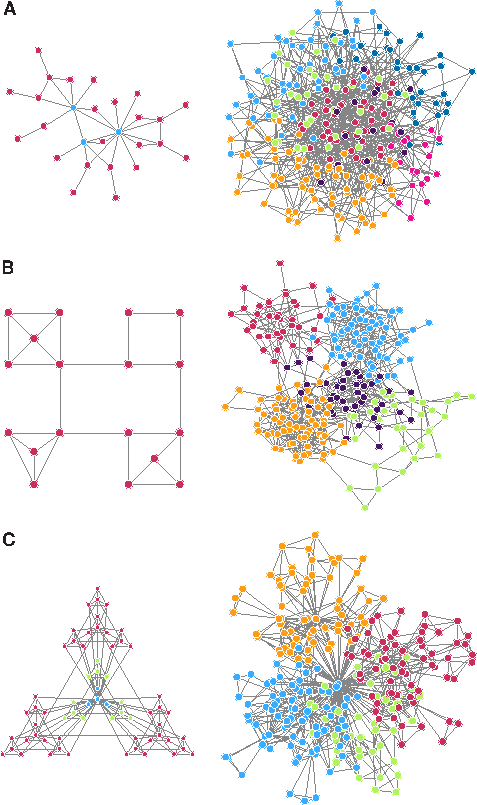
\includegraphics[width=0.57\textwidth]{img/intro/3_coexpr/intro_3_coexpr_ravasz_hierarchical_clustering.pdf}
    \caption[Modèles de réseaux complexes, issus et traduits de Ravasz \textit{et al.}]{Modèles de réseaux complexes, issus et traduits de Ravasz \textit{et al.} \cite{Ravasz2002} et adaptés pour être compatible au daltonisme. \textbf{(A)} Illustration schématique (à gauche) d'un réseau à invariance d'échelle, dont la distribution des degrés suit une loi de puissance. Dans un tel réseau, quelques nœuds fortement connectés, ou hubs (cercles bleus), jouent un rôle important pour maintenir la cohésion de l'ensemble du réseau. Une configuration typique (à droite) d'un réseau sans échelle de 256 nœuds est également illustrée, obtenue à l'aide du modèle à invariance d'échelle, qui requiert l'ajout d'un nouveau nœud à chaque fois de sorte que les nœuds existants ayant des degrés de connectivité plus élevés ont plus de chances d'être liés aux nouveaux nœuds \cite{Barabasi1999Oct}. Les nœuds sont disposés dans l'espace à l'aide d'un algorithme de partitionnement standard \cite{Batagelj1998} pour illustrer l'absence de modularité sous-jacente. \textbf{(B)} Illustration schématique (à gauche) d'un réseau manifestement modulaire composé de quatre modules fortement interconnectés et reliés entre eux par quelques liens. Cette topologie intuitive n'a pas de distribution de degrés sans échelle, car la plupart de ses nœuds ont un nombre similaire de liens, et les hubs sont absents. Un algorithme de partitionnement standard révèle la modularité inhérente du réseau (à droite) en partitionnant un réseau modulaire de N = 256 nœuds en quatre structures isolées intégrées au système. \textbf{(C)} Le réseau hiérarchique (à gauche) présente une topologie d'invariance d'échelle avec une modularité intégrée. Les niveaux hiérarchiques sont représentés par ordre croissant de bleu à vert et rouge. Les algorithmes de partitionnement standard (à droite) ne parviennent pas à mettre en évidence la modularité sous-jacente du réseau. Une caractérisation quantitative détaillée des trois modèles de réseau est disponible dans www.nd.edu/~networks/cell/index.html\footnotemark.}
    \label{fig:ravasz_hierarchical_clustering}
\end{figure}

Ainsi, les gènes au sein d'un réseau vont avoir tendance à s'organiser sous forme de multiples groupes de gènes, des \glspl{module}, formant eux-mêmes des modules plus importants. L'origine biologique de ce type d'organisation est l'objet de nombreuses hypothèses sans qu'aucune n'ait pu être estimée plus plausible qu'une autre \cite{Lorenz2011}. Une forte co-expression locale est présente et on y retrouve des \textbf{gènes pivot intra-modules} qui centralisent la majorité des plus courts chemins. Les modules sont également reliés entre eux par un faible nombre de \textbf{gènes pivot inter-modules} qui font office de passerelle.
% Les genes intramodule sont interessants, techniquement pas les inter  % doi.org/10.1371/journal.pone.0061505 + 

\footnotetext{Lien originel inclut dans la publication. Renvoi aujourd'hui une erreur "404 - page inconnue"}

Pour prendre en compte cette topologie en vue de faciliter la détection de gènes, S. Horvath et B. Zhang proposent alors d'ajouter une surcouche à l'adjacence calculée. En se basant sur les travaux de Ravasz \textit{et al.}, ils implémentent le score de recouvrement topologique qui va mesurer l'inter-connectivité relative de deux nœuds (Équation \ref{topological_overlap_eq}, Figure \ref{fig:topological_overlap_schema}) dans leur calcul du score de similarité. Ils vont cependant faire le choix de passer d'un score de similarité à un score de dissimilarité (Équation \ref{dissimilarity_to}). 

\begin{align} 
    \omega_{i j} &= \frac{l_{i j}+a_{i j}}{\min \left\{k_{i}, k_{j}\right\}+1-a_{i j}} \label{topological_overlap_eq} \\ 
    d_{i j}^{\omega} &= 1-\omega_{i j} \label{dissimilarity_to}
\end{align}
Où :
\begin{align*}
    a_{i j} & = \text{adjacence} \\
    l_{i j} &= \sum_{u} a_{i u} a_{u j} \\
    k_{i} &= \sum_{u} a_{i u} = \text{connectivité ou force du nœud}
\end{align*}

\begin{figure}[ht]
    \centering
    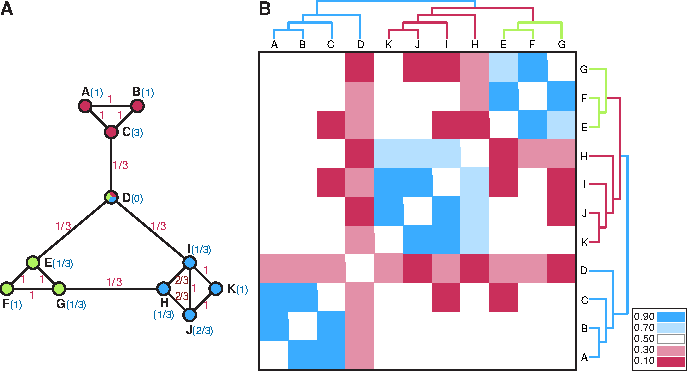
\includegraphics{img/intro/3_coexpr/intro_3_coexpr_ravasz_topological_overlap.pdf}
    \caption[Découverte de la modularité sous-jacente d'un réseau complexe]{Découverte de la modularité sous-jacente d'un réseau complexe, issu de Ravasz \textit{et al.} \cite{Ravasz2002} et adaptés pour être compatible avec le daltonisme. \textbf{(A)} Recouvrement topologique illustré sur un petit réseau hypothétique. Pour chaque paire de nœuds, $i$ et $j$, nous définissons le recouvrement topologique $O_T(i, j) = J_n(i, j)/[min (k_i,k_j)]$, où $J_n(i, j)$ désigne le nombre de nœuds auxquels $i$ et $j$ sont liés (+ 1 s'il existe un lien direct entre $i$ et $j$) et $[min (k_i,k_j)]$ est le plus petit des degrés $k_i$ et $k_j$. Sur chaque lien, nous indiquons le recouvrement topologique pour les nœuds connectés, et entre parenthèses à côté de chaque nœud, nous indiquons le coefficient de partitionnement du nœud. \textbf{(B)} La matrice de recouvrement topologique correspondant au petit réseau présenté en (A). Les lignes et les colonnes de la matrice ont été réorganisées par l'application d'une méthode de partitionnement par liaison moyenne \cite{Eisen1998Dec} à ses éléments, ce qui nous permet d'identifier et de placer à proximité les uns des autres les nœuds qui présentent un recouvrement topologique élevé. Le code couleur indique le degré de recouvrement topologique entre les nœuds. L'arbre associé reflète les trois modules distincts construits dans le modèle en (A), ainsi que le fait que les modules EFG et HIJK sont plus proches les uns des autres au sens topologique que le module ABC.}
    \label{fig:topological_overlap_schema}
\end{figure}

Le score de similarité qui en résulte est donc une métrique de la concordance entre les voisins directs de deux nœuds. Par la suite, d'autres améliorations ont également été proposées comme l'utilisation d'un score de recouvrement topologique généralisé \cite{Yip2007Dec} ou encore une implémentation différente du recouvrement de topologie, wTO \cite{Gysi2018}, pour pouvoir lui associer une \textbf{valeur p}. Chacun de ces scores ayant ses propres avantages et limites, le choix de l'un ou l'autre pour la construction d'un réseau reposera avant tout sur la question de recherche. wTO est ainsi meilleur pour étudier les réseaux dans lesquels il est important de savoir si une interaction est activatrice ou inhibitrice/répressive. Le score de S. Horvath et B. Zhang présente lui une comparabilité accrue avec d'autres méthodes de construction de réseaux de co-expression aux métriques non signées. Une fois le score adapté choisi, il est enfin possible de détecter plus facilement les modules de co-expression.



\subsection{Détection de modules}

\subsubsection{Point sur les méthodes}

Le module est l'unité majeure d'interprétation des \acrshort{GCN}. En effet, il regroupe des gènes au profil d'expression similaire au sein de plusieurs échantillons car ceux-ci tendent à être impliqués dans des fonctions physiologiques communes ou des \glspl{phenotype} définis. La détection des modules vise donc à grouper les gènes dans le réseau en tenant compte des scores de similarité des gènes. Face au défi qu'est l'identification d'unités fonctionnelles dans des réseaux de régulation biologique complexes et chevauchants, de nombreuses méthodes ont été utilisées sont classables en plusieurs catégories (Figure \ref{fig:category_detection_module}) \cite{Saelens2018} : 
\begin{itemize}
    \item Partitionnement : regroupement de gènes sur la base d'un score de similarité globale issu de la matrice d'\glspl{genexpr}.
    \item Décomposition : extraction des composants correspondant aux modules de co-expression en décomposant la matrice d'expression en un produit de matrices plus petites.
    \item Bi-partitionnement : regroupement simultané de gènes et d'échantillons en classification double sur la base d'un comportement local similaire en matière d'expression.
    \item Inférence de réseau itérative : optimisation itérative d'un réseau inféré et d'un ensemble de partitions.
    \item Inférence de réseau directe : inférence d'un réseau de régulation basé sur la similarité de l'expression génétique entre les régulateurs et les gènes cibles.
\end{itemize} 
\hfill

\begin{figure}[ht]
    \centering
    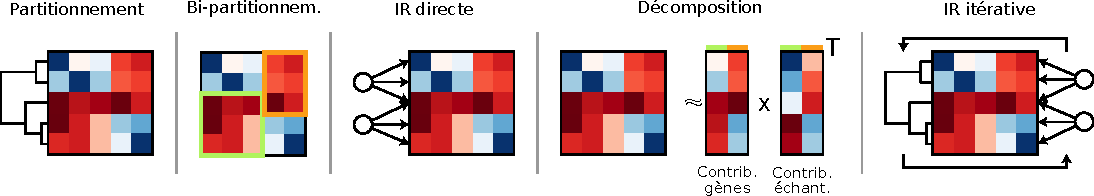
\includegraphics[width=\textwidth]{img/intro/3_coexpr/intro_3_coexpr_category_detection_module.pdf}
    \caption[Illustration des 5 catégories de méthodes de détection de modules.]{Illustration des 5 catégories de méthodes de détection de modules. Extrait de Saelens \textit{et al.} 2018 (CC-BY) \cite{Saelens2018} et adapté pour être compatible au daltonisme. IR = Inférence de réseau.}
    \label{fig:category_detection_module}
\end{figure}

La détection de modules servant différents objectifs, certaines approches sont plus adaptées que d'autres dépendant de la question de recherche. Dans la majorité des cas, la détection de modules peut permettre d'avoir un aperçu global des données sans apport de connaissances extérieures comme des voies d'activations, d'identifier des fonctions biologiques ou des maladies et d'inférer des réseaux de régulation. La méthode par partitionnement permettant de répondre à tous ces besoins \cite{Filteau2013,Sundarrajan2016,Kogelman2014} et étant encore à ce jour la plus utilisée \cite{Saelens2018}, c'est sur elle qu'on s'est concentré dans cette thèse.

\subsubsection{Partitionnement hiérarchique}

\begin{figure}[b]
    \centering
    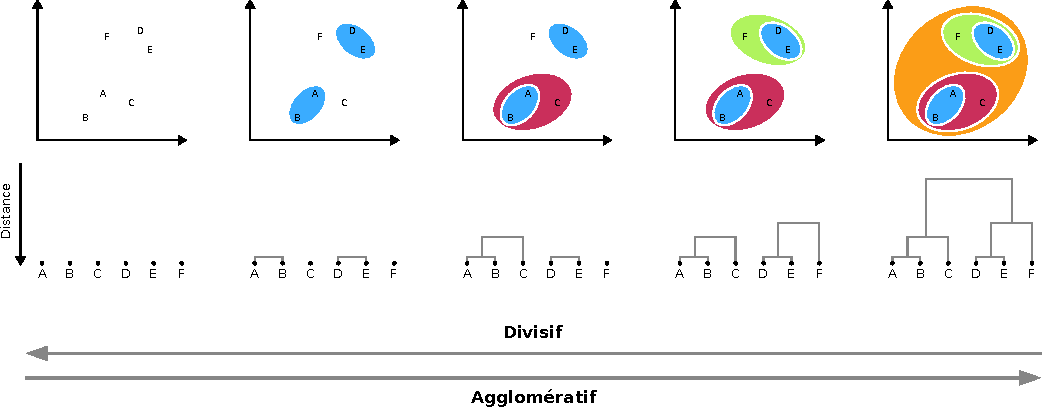
\includegraphics[width=\textwidth]{img/intro/3_coexpr/intro_3_coexpr_hierarchical_clustering.pdf}
    \caption{Principe du partitionnement hiérarchique. Chacun des 6 points du nuage est associé à chaque étape avec le point le plus proche dans un groupe. L'arbre est ensuite coupé traditionnellement pour obtenir les groupes, dans le cas de la co-expression, les modules.}
    \label{fig:my_label}
\end{figure}

Les méthodes de partitionnement sont variées mais seules trois semblent être utilisées en majorité dans la recherche se servent des réseaux de co-expression : le partitionnement par connectivité, le partitionnement par centroïdes, et le partitionnement par distribution. Si ces deux dernières méthodes ont fait leurs preuves pour détecter des modules d'intérêt \cite{Ruan2006Dec,Shi2010Dec, Rau2018}, le partitionnement par connectivité, aussi appelé partitionnement hiérarchique reste une procédure largement utilisée \cite{Tang2018, Mao2009, Rotival2013}. Il est apprécié pour son compromis entre facilité d'implémentation, pertinence des modules détectés, et besoins en ressources tant en temps qu'en puissance de calcul \cite{Saelens2018}. Il est également particulièrement adapté aux réseaux biologiques qui suivent une topologie modulaire hiérarchique comme ceux de gènes. 

La méthode initiale \cite{Murtagh2012Jan} consiste à construire un arbre de distances (un dendrogramme) en calculant un critère de liaison entre chaque point. Chaque point et ensuite soit regroupé itérativement selon les points les plus proches (processus agglomératif), soit divisé en deux groupes à chaque tour les points (processus divisif). L'arbre final est coupé selon un seuil qui va définir les points regroupés ensemble, dans notre cas les gènes regroupés dans un même module. Ce seuil ayant été plusieurs fois critiqué pour son côté trop statique dans la hauteur de découpe et son côté arbitraire, une amélioration consiste à rendre le seuil dynamique \cite{Langfelder2008_cutree}. Pour cela, les branches du dendrogramme sont analysées à la recherche de structures de sous partitions récursivement jusqu'à une stabilisation des sous clusters. Cette approche permet donc une définition de clusters de hauteur différente dans le dendrogramme pour chaque branche.

Ces méthodes de construction et de détection des modules sont finalement celles implémentées dans le populaire progiciel (en anglais \textit{package}) R WGCNA créé par P. Langfelder et S. Hortvath \cite{Langfelder2008}. Développé en 2008, ce progiciel a permis de démocratiser l'analyse par réseaux de co-expression et de donner des modules prêts à être interprétés. Pour leur donner tout leur sens, il est cependant nécessaire d'effectuer des analyses supplémentaires.



\subsection{Exploitation des modules de gènes}

\subsubsection{Approche guidée par la connaissance préalable : l'intégration biologique}

Les modules tendent à regrouper des gènes aux fonctions physiologiques semblables ou co-régulés \cite{Barabasi2011Jan,Lorenz2011}. Une façon de comprendre la raison du regroupement de ces gènes est donc de leur rattacher une fonction, une voie d'activation, un tissu ou une maladie dans laquelle ils interviennent. Cette approche est alors qualifiée de guidée par la connaissance préalable (en anglais \textit{knowledge-driven}). Cependant, les gènes œuvrant rarement à une seule fonction, ils se retrouvent annoté de plusieurs fonctions \cite{Green2006Aug} plus ou moins pertinentes dans le contexte du module. Pour estimer lesquelles sont réellement significatives dans chaque module, on effectue donc des analyses d'enrichissement \cite{Khatri2012} par rapport à diverses sources d'annotations (Table \ref{table:common_enrich_sources}). Appelée également par raccourci analyse de voies d'activation (en anglais \textit{pathway analysis}), cette analyse peut être effectuée de trois façons dépendamment des méta-données disponibles : l'analyse de sur ou sous représentation, la cotation de classe fonctionnelle, et l'approche basée sur la topologie des voies d'activation. 


\begin{table}[ht]
\resizebox{\textwidth}{!}{
\begin{tabular}{@{}llll@{}}
\toprule
\textbf{Source de données}                                                                          & \textbf{Acronyme} & \textbf{Description}                                                                                                                                                                                                                                        & \textbf{Compatible PT ?} \\ \midrule
Gene Ontology                                                                                       & GO                & \begin{tabular}[c]{@{}l@{}}Modèle informatique de systèmes biologiques sous forme \\ d'ontologie décrivant des fonctions physiologiques, \\ moléculaires et cellulaire de différents organismes\end{tabular}                                                & oui                      \\
\begin{tabular}[c]{@{}l@{}}Kyoto Encyclopedia of \\ Genes and Genomes\end{tabular}                  & KEGG              & \begin{tabular}[c]{@{}l@{}}Ensemble de bases de données relatives aux génomes, aux \\ voies métaboliques et aux composés biochimiques, associées \\ à une représentation en réseau des intéractions moléculaires\end{tabular}                               & oui                      \\
Reactome                                                                                            & Reactome          & \begin{tabular}[c]{@{}l@{}}Processus biologiques humains annotés sous la forme d'une \\ série d'événements moléculaires imbriqués\end{tabular}                                                                                                              & oui                      \\
WikiPathways                                                                                        & WP                & \begin{tabular}[c]{@{}l@{}}Ressource communautaire pour la contribution et la \\ maintenance de contenu dédié aux voies d'activation \\ métaboliques\end{tabular}                                                                                           & oui                      \\
\begin{tabular}[c]{@{}l@{}}MicroRNA-Target \\ Interactions database\end{tabular}                    & mirTarBase        & \begin{tabular}[c]{@{}l@{}}Base de données revue des interactions micro ARN et \\ séquence cible\end{tabular}                                                                                                                                               & non                      \\
TRANSFAC                                                                                            & TRANSFAC          & \begin{tabular}[c]{@{}l@{}}Ressource de facteurs de transcriptions, sites de liaisons et \\ éléments régulés\end{tabular}                                                                                                                                   & non                      \\
\begin{tabular}[c]{@{}l@{}}Comprehensive Resource \\ of Mammalian \\ protein complexes\end{tabular} & CORUM             & \begin{tabular}[c]{@{}l@{}}Collection de complexes protéiques chez les mammifères \\ expérimentalement vérifiés\end{tabular}                                                                                                                                & non                      \\
Human Protein Atlas                                                                                 & HPA               & \begin{tabular}[c]{@{}l@{}}Cartographie de l'ensemble des protéines humaines par type \\ cellulaire, tissu, organe\end{tabular}                                                                                                                             & non                      \\
\begin{tabular}[c]{@{}l@{}}Human Phenotype \\ Ontology\end{tabular}                                 & HPO               & \begin{tabular}[c]{@{}l@{}}Modèle informatique de systèmes biologiques sous forme \\ d'ontologie décrivant des phénotypes humains\\ anormaux et/ou associés à des maladies\end{tabular}                                                                     & oui                      \\
\begin{tabular}[c]{@{}l@{}}Molecular Signatures \\ Database\end{tabular}                            & MSigDB            & \begin{tabular}[c]{@{}l@{}}Ensemble de 9 collections d'annotations sur la localisation \\ chromosomique, les voies métaboliques, la régulation, les \\ signatures oncologique, l'immunologie, le type cellulaire, \\ et différentes ontologies\end{tabular} & non                      \\ \bottomrule
\end{tabular}
}
\caption[Sources d'enrichissement communes en analyse d'enrichissement]{Sources d'enrichissement communes en analyse d'enrichissement. PT = approche basée sur la topologie des voies d'activation}
\label{table:common_enrich_sources}
\end{table}


En l'absence d'autres données que les identifiants de gènes, on peut effectuer une analyse de sur ou sous représentation (en anglais \textit{over-representation analysis} ou ORA) par rapport à un contexte et une source d'annotation donnée \cite{Khatri2012}. Par exemple, on pourra chercher si un ensemble d'identifiants de gènes issus d'un module est sur-représenté par rapport à la normale dans groupe de gènes annotant une voie métabolique sur l'ensemble des gènes chez l'humain (Figure \ref{fig:enrichment_methods}). Pour estimer si la sur-représentation est significative, on utilise le plus souvent un test hyper-géométrique bien que d'autres distributions comme le chi\textsuperscript{2} ou la binomiale soient également utilisés plus occasionnellement \cite{Huang2009Jan}. Le test étant répété pour de nombreuses annotations, une correction pour test multiple doit être réalisée. L'inconvénient majeur de l'enrichissement par sur-représentation réside dans sa pondération uniforme de l'impact de chaque gène, ce qui est loin de représenter la réalité biologique qui est hiérarchique \cite{Khatri2012}.

Si en plus des identifiants de gènes on possède un score, par exemple un poids, un taux de variation, un rang, une valeur p, on peut effectuer une cotation de classe fonctionnelle (en anglais \textit{functional class scoring} ou FSC), aussi appelée de façon confondante analyse d'enrichissement de collection de gènes (en anglais \textit{gene set enrichment analysis} ou GSEA). Le score à considérer pour les gènes va impacter fortement les enrichissements obtenus \cite{Ackermann2009Dec} et doit donc être choisi avec précaution. Pour obtenir l'enrichissement, la cotation de classe fonctionnelle va tout d'abord calculer une statistique au niveau des gènes (ex: valeur p, un rang, un taux de fausses découvertes), si le score fournit n'est pas déjà de cette nature. Ces statistiques de niveau de gènes sont ensuite agglomérées par source d'annotation donnée selon une méthode de résumé de l'information comme une médiane, une statistique de Kolmogorov-Smirnov, ou une somme de rang de Wilcoxon \cite{Khatri2012}. Finalement, cette statistique agglomérée est testée pour sa significativité par test de permutation ou de comparaison au hasard (Figure \ref{fig:enrichment_methods}). Si cette méthode répond à la limitation des tests de sur-représentation évoqués plus haut, elle possède elle-même une limite majeure car elle considère les annotations données de façon indépendante. Les annotations se chevauchant régulièrement du fait de l'implication récurrente d'un gène dans plusieurs annotations, un biais est nécessairement présent.

La méthode d'enrichissement la plus récente est l'approche basée sur la topologie des voies d'activation (en anglais \textit{pathway topology based approache} ou PT). Cette méthode prend en compte non pas juste une liste d'identifiants de gènes et leur score associé, mais les liens existants entre les gènes dans les sources d'annotation \cite{Khatri2012} (Table \ref{table:common_enrich_sources}). Ainsi, si une voie métabolique se voit changer l'agencement des liens entre les différents gènes, sans pour autant changer la liste des gènes, l'approche par topologie des voies d'activation sera capable d'en tenir compte dans son résultat d'enrichissement contrairement aux deux méthodes précédentes. Son fonctionnement est similaire à celui de la cotation par classe fonctionnelle qui, à la différence que la statistique de niveau de gène telle que ScorePAGE \cite{Rahnenfuhrer2004Jun} calcule un niveau de similarité entre chaque paire de gènes de l'annotation donnée et le divise par le nombre de réactions nécessaires pour connecter les deux gènes (Figure \ref{fig:enrichment_methods}). L'apport d'information supplémentaire permet donc de préciser encore plus les enrichissements obtenus. Toutefois, cette méthode requière des sources d'annotation possédant des liens entre les gènes donnés, et celles-ci ne représentent qu'un faible nombre de sources.

\begin{figure}
    \centering
    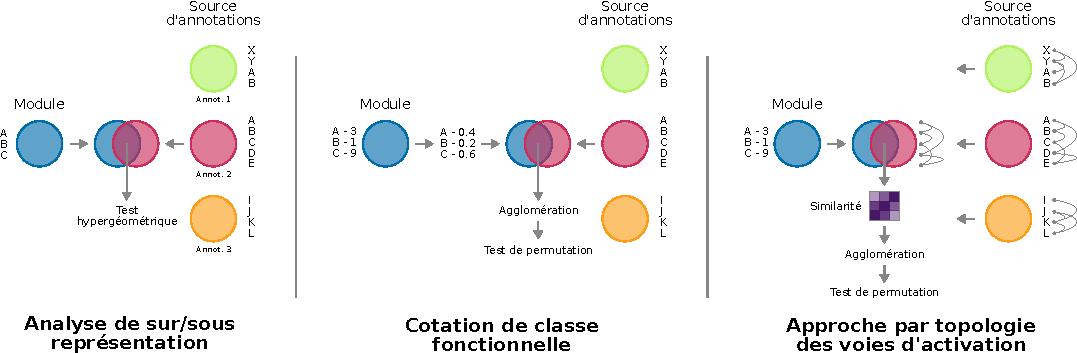
\includegraphics[width=\textwidth]{img/intro/3_coexpr/intro_3_coexpr_enrichment_methods.pdf} 
    \caption[Schématisation des différentes méthodes d'enrichissement de groupes de gènes.]{Schématisation des différentes méthodes d'enrichissement de groupes de gènes. Le module composé des gènes A,B,C est dans chacun des 3 exemples enrichit selon une source d'annotation contenant trois annotations au nombre de gènes variables. Dans le cas de l'analyse de sur ou sous représentation, seuls les identifiants sont fournis coté module. Dans la cotation fonctionnelle de classe et l'approche par topologie de voie d'activation, des scores sont en plus associés aux gènes du module. Dans le cas de l'approche par topologie de voie d'activation, des informations sur les liens entre les différents gènes des annotations est en plus fournit.}
    \label{fig:enrichment_methods}
\end{figure}


En plus des tests d'enrichissement qui apportent une information généraliste par le biais des sources d'annotations, on peut apporter une information plus spécifique si des \glspl{phenotype} sont fournis pour les échantillons via les tests d'association phénotypique \cite{Langfelder2008}. Afin de tester chaque module avec chaque phénotype, on cherche tout d'abord à représenter chaque module sous une forme moyenne. Pour ce faire, on effectue une décomposition en valeurs singulières de l'\glspl{genexpr} contenus dans un module, et on sélectionne la première composante calculée qu'on nommera gène propre (en anglais \textit{eigengene}). Dans le cas de variables quantitatives comme l'âge, la taille, le poids, il est directement possible d'effectuer un test de corrélation avec le gène propre d'un module pour déterminer si celui-ci est significativement associé à la variable phénotypique considérée. Dans le cas d'une variable qualitative, il est nécessaire de la binariser pour pouvoir effectuer l'association avec le gène propre \cite{Lemoine2021Dec}. Cette technique consiste transformer chaque modalité de la variable en une variable à part entière dont la valeur sera 1 lorsque l'échantillon possède cette modalité, et 0 pour le reste de la variable ainsi que les autres variables modales (Figure \ref{fig:binarisation}).

\begin{figure}[ht]
    \centering
    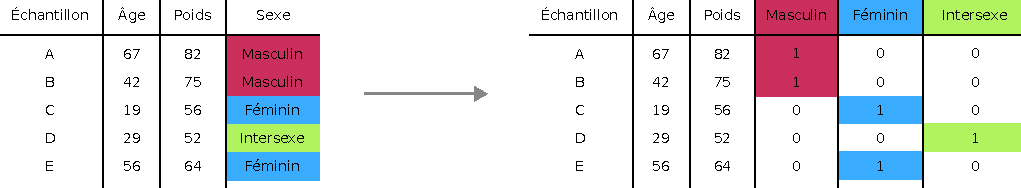
\includegraphics[width=\textwidth]{img/intro/3_coexpr/intro_3_coexpr_binarisation.pdf}
    \caption[Exemple de binarisation de variable catégorielle]{Exemple de binarisation de variable catégorielle. La variable du sexe comportant 3 modalités, homme, femme, et intersexe est transformée en 3 variables distinctes qui codent pour les catégories initiales par des valeurs binaires.}
    \label{fig:binarisation}
\end{figure}

Ces différentes approches guidées par la connaissance permettent finalement d'effectuer des prédictions fonctionnelles \textit{in silico} quand associées à l'analyse de \acrshort{GCN}. Le paradigme de l'association par culpabilité (en anglais \textit{guilt by association}) présume en effet que des gènes fortement co-exprimés, comme ceux présents dans les modules, contribuent ou partagent de mêmes fonctions physiologiques\cite{Ballouz2015}. Cette association est donc particulièrement utile pour l'annotation de gènes qui sont peu ou pas étudiés en se basant sur les enrichissements et associations phénotypiques obtenus \cite{Wolfe2005}. Il faut toutefois noter que si l'ajout de connaissances établies permet d'acquérir de nouvelles connaissances et de comprendre le contexte biologique dans lequel se situent des modules, il apporte aussi avec lui un risque de biais. Les sources d'enrichissement sont par exemple disproportionnées concernant certains gènes ou familles de gènes \cite{Timmons2015Dec}. L'utilisation conjointe de méthodes dites guidées par les données (en anglais \textit{data-driven}) est donc un moyen de compléter de façon moins biaisée l'interprétation des modules.


%%\subsection{Capitalisation sur l'information intrinsèque aux données}
% \subsubsection{Approche guidée par les données : l'étude statistique et topologique}
\subsubsection{Approche guidée par les données : l'étude topologique}

Les motifs d'organisation et les structures présentes dans un réseau sont depuis longtemps étudiés dans une volonté de rattacher ensemble topologie et fonction biologique. Les gènes concentrant les liens dans un réseau les gènes pivot, étant des structures facilement notables, elles ont été étudiées très tôt. Les gènes pivot ont ainsi été trouvés associés à des gènes essentiels à la survie d'un \gls{organisme} \cite{Jeong2001May}. Une analyse de ces gènes pivot croisée aux gènes responsables de maladies Mendéliennes a cependant écarté l'hypothèse intuitive que les gènes pivot étaient la clef de ces maladies mono-géniques\cite{Goh2007May}. À la place, les gènes associés à ces maladies et aux maladies non-Mendéliennes ont plutôt été retrouvés en périphérie ou à des positions neutres du réseau \cite{Jeong2001May}. La détection des gènes pivot reste donc intéressante pour favoriser la détection de gènes aux fonctions essentielles ou bien celle de gènes potentiellement liés à une maladie, dans le cas de l'étude de gènes \glspl{voisin} \cite{Langfelder2013}.

La méthode de détection des gènes pivot a toutefois souffert d'une définition assez vague de ce que sont les gènes pivot. On retrouve ainsi des définitions telles que sélectionner les dix gènes les plus connectés \cite{Russo2018}, un pourcentage de gènes les plus connectés et une façon de mesurer cette connectivité qui varie selon l'étude \cite{Sundarrajan2016, Tang2018} ou encore un métrique de théorie des réseaux seuillée arbitrairement \cite{Saha2017}. Deux mesures parmi celles existantes ressortent pour leur définition de gènes pivots basé uniquement sur la topologie et un test statistique, sans seuil extérieur :
\begin{itemize}
    \item La sur-connectivité \cite{Das2017} : la connectivité, c’est-à-dire la somme des poids des liens d'un nœud, et testée statistiquement par rapport à la connectivité moyenne du réseau pour estimer si la différence est significative. Le degré est aussi parfois utilité comme mesure initiale.
    \item L'adhésion au module \cite{Horvath2008} : la corrélation entre l'expression d'un gène et le gène propre d'un module est testée pour estimer sa significativité.
\end{itemize}

Plus précisément encore, ce type de mesure va permettre de détecter des gènes pivots dit intra-module (Figure \ref{fig:hub_gene_intra_inter}). D'autres gènes possèdent une structure de pivot mais se placent plutôt en passerelle entre les modules ou sous-modules du réseau lié à la topologie hiérarchique. Ceux-ci sont détectables par une analyse des nœuds les plus présents dans les plus courts chemins pour parcourir le réseau d'un nœud à un autre (Figure \ref{fig:hub_gene_intra_inter}). Leur implication et caractérisation biologique reste toutefois encore peu étudiée.

\begin{figure}[hb]
    \centering
    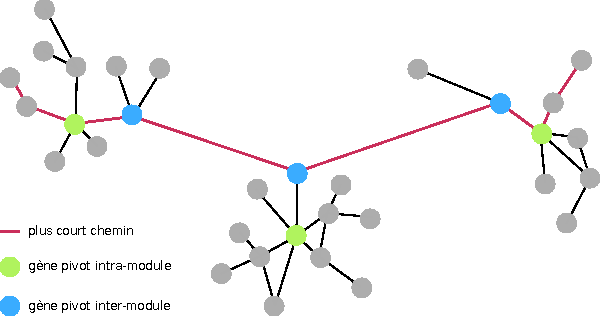
\includegraphics{img/intro/3_coexpr/intro_3_coexpr_hub_gene.pdf}
    \caption[Réseau illustrant la topologie présentée par les gènes pivot intra et inter-modules]{Réseau illustrant la topologie présentée par les gènes pivot intra et inter-modules. Les gènes pivot intra-module (en vert) sont centraux au sein des modules. Les gènes pivot inter-modules (en bleu) sont le lieu de passage d'une grande quantité de plus courts chemins (en rouge).}
    \label{fig:hub_gene_intra_inter}
\end{figure}



\subsubsection{Comparaison de réseaux entre conditions : la co-expression différentielle}

Les comparaisons sain contre malade, sauvage contre muté, ou toute autres \glspl{condition} contrôle contre test ont toujours été une approche de choix pour comprendre les altérations d'une condition en biologie. Les \acrshort{GCN} n'échappent pas à la règle et des méthodes de comparaison de réseau sont rapidement apparues \cite{Lai2004Nov}. L'analyse de co-expression différentielle (en anglais \textit{differential co-expression} ou DCE) est complémentaire de l'analyse classique d'expression différentielle en détectant les gènes dont les motifs de régulation changent sans que l'\glspl{genexpr} varie elle-même significativement. Certains gènes associés à des maladies ont en effet un niveau d'expression constant mais avec une modification du transcrit telle qu'une mutation, un épissage alternatif, ou une altération post-transcriptionnelle qui vont venir affecter sa fonction \cite{delaFuente2010Jul}. Ce phénomène est observable dans le cas de perturbation d'éléments de régulation \cite{Rotival2013}, dans le cas de comparaisons de tissus \cite{Gov2017}, ou entre espèces similaires voir \glspl{organisme} \cite{Chowdhury2019}.


\begin{table}[b]
\resizebox{\textwidth}{!}{
\begin{tabular}{@{}ll@{}}
\toprule
\textbf{Name}                                                                               & \textbf{Description}                                                                                \\ \midrule
\multirow{2}{*}{Density}                                                                    & It measures compactness of a module. Density is defined as the average connection strength of       \\
                                                                                            & all pairs of genes present in a module.                                                             \\
\multirow{2}{*}{Clustering coefficient}                                                     & Clustering co-efficient of a node quantifies the interconnectedness of its neighboring nodes. The   \\
                                                                                            & average of clustering coefficients of all nodes measures the modularity of a module.                \\
\multirow{5}{*}{Maximum adjacency ratio}                                                    & It generally deals with a weighted network and can be used to check whether a hub gene is           \\
                                                                                            & connected to a large number of genes with moderate connection strengths or a few genes with         \\
                                                                                            & strong connection strengths \cite{Horvath2008}. By computing the average MAR, we can distinguish among       \\
                                                                                            & the connectivity patterns. More the correlation between MAR of nodes in two modules across          \\
                                                                                            & conditions, then the preservation is higher.                                                        \\
\multirow{3}{*}{\begin{tabular}[c]{@{}l@{}}Sign preserving mean\\ correlation\end{tabular}} & This module preservation strategy takes element-wise multiplication of the correlation matrices     \\
                                                                                            & for the same module in two different samples groups and then takes the mean. Higher mean            \\
                                                                                            & means more preservation.                                                                            \\
\multirow{3}{*}{Eigengene based measure}                                                    & Eigengene is an arbitrary gene represents a module very well. To calculate preservation, one        \\
                                                                                            & can take the correlation between the eigengenes of the corresponding modules of different           \\
                                                                                            & phenotypes. Higher correlation means more preservation.                                             \\
\multirow{3}{*}{Intra-modular connectivity}                                                 & The sum of connection strengths of neighbors of a node. To investigate preservation,                \\
                                                                                            & correlation of intra-modular connectivity of nodes present in the same module of different          \\
                                                                                            & phenotypes can be used. More correlation implies higher preservation.                               \\
\multirow{2}{*}{Fitting coefficient (R2) \cite{Zhang2005a}}                                          & Scale-free topology criteria of a network can be quantified using the fitting coefficient of linear \\
                                                                                            & regression.                                                                                         \\
\multirow{2}{*}{Global network connectivity \cite{Taylor2009Feb}}                                      & This characteristic path length is the average of the shortest paths between all pairs of nodes in  \\
                                                                                            & a network.                                                                                          \\
\multirow{2}{*}{Zsummary \cite{Langfelder2011}}                                                         & It quantifies the amount of preservation of a module of reference in a test network by              \\
                                                                                            & considering density and connectivity of that module in both networks.                               \\
\multirow{2}{*}{MedianRank \cite{Langfelder2011}}                                                       & It gives the ranking of a reference network modules in a test network. The most preserved           \\
                                                                                            & module gets the top rank.                                                                           \\ \cmidrule(l){2-2} 
\end{tabular}
}
\caption[Statistiques pour la préservation des modules et la mesure des perturbations]{Statistics for Module Preservation and Disruption Measurement. Statistiques pour la préservation des modules et la mesure des perturbations. Issu de Chowdhury \textit{et al.} \cite{Chowdhury2019} \textcopyright 2019 IEE. Traduction non autorisée.}
\label{table:chowdury_metrics_DCE}
\end{table}


Réaliser une analyse DCE demande cependant un regard critique sur les données utilisées en entrée tout comme sur la méthode de co-expression différentielle employée. Des différences individuelles de liens ou du poids dans le réseau ne sont ainsi pas suffisantes à elles seules pour indiquer une divergence de fonction et pourraient être le fruit de biais techniques, par exemple de la méthode de séquençage \cite{Southworth2009}. De la même manière que pour l'expression différentielle classique, il faut s'assurer de la significativité des changements de motif observés. Face à la diversité d'observations possibles, plusieurs méthodes ont vue le jour avec l'influence tant de la théorie des réseaux que de la biostatistique (Table \ref{table:chowdury_metrics_DCE}. Initialement partis d'une simple comparaison de l'expression moyenne par nœuds ou jusqu'à un nombre défini de nœuds voisins, les méthodes de co-expression différentielle ont évolué pour s'orienter sur de la détection de modifications de motifs complexes dans un réseau \cite{delaFuente2010Jul}. 

Les variations singulières de gènes en DCE sont généralement le reflet de maladies Mendéliennes ou de traits phénotypiques monogéniques. Pour investiguer des conditions polygéniques, on utilise plus souvent l'échelle du module pour investiguer les différences de co-expression entre deux conditions. On parle alors d'analyse de préservation ou non préservation des modules de co-expression entre des conditions. De façon similaire à l'interprétation des modules qui peut se faire via des détections de voies d'activation ou via de la topologie, la co-expression différentielle peut reconnaître les modules préservés ou non préservés en étudiant la conservation de voies d'activation ou de motifs de liens au sein du module \cite{Chowdhury2019}. Face à la diversité de changement de topologie, l'analyse par modification des liens requière toutefois plus de détail qu'une analyse présence/absence des comparaisons d'enrichissement. On peut ainsi observer des disparitions totales de modules, des variations de leur composition en gène, des séparations d'un module en plusieurs ou inversement, des changements de co-expression par grappe (Figure \ref{fig:differential_coexpression_patterns}).

\begin{figure}[hb]
    \centering
    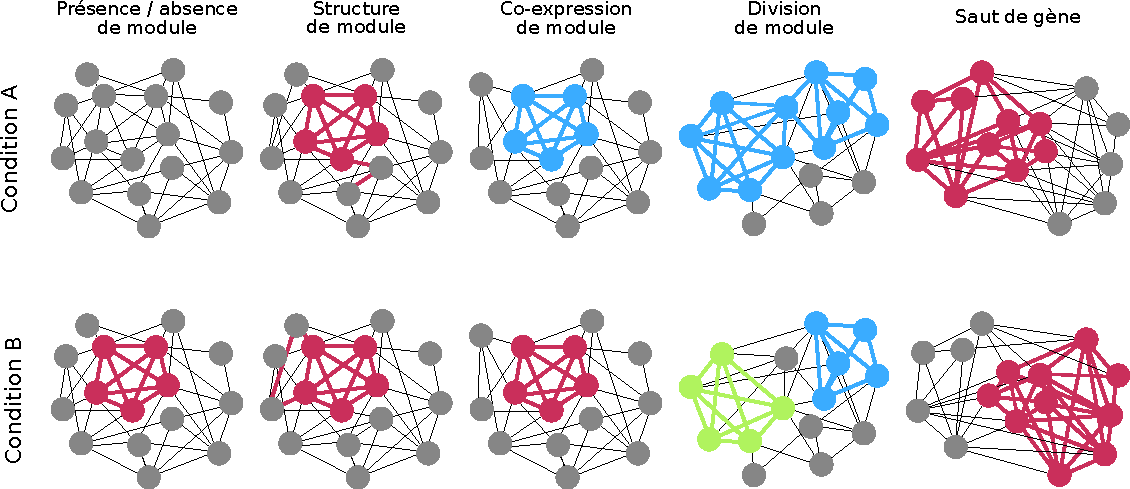
\includegraphics[width=\textwidth]{img/intro/3_coexpr/intro_3_coexpr_codiff.pdf}
    \caption[Motifs de changements de co-expression entrainant une non-préservation des modules dans une analyse de co-expression différentielle]{Motifs de changements de co-expression entrainant une non-préservation des modules dans une analyse de co-expression différentielle. D'après Van Dam \textit{et al.} \cite{VanDam2018} et adaptés pour être compatible au daltonisme. Les motifs peuvent consister en une apparition ou disparition de module en raison des changement d'intensité de corrélation, une modification partielle des gènes inclus dans le module, une variation globale de l'intensité de co-expression sans changer la conformation du module comme une diminution de tous les liens, une séparation en deux d'un module initial ou une jointure de deux modules initiaux, un saut de la co-expression d'un sous groupe de gène vers un autre groupe en raison notamment de la présence de facteurs de transcription.}
    \label{fig:differential_coexpression_patterns}
\end{figure}



En 2005 lors de la publication de leur méthode d'analyse par co-expression, B. Zhang et S. Horvath présentent également sept métriques de caractérisation de la topologie d'un réseau (Annexe \ref{annexe:supp_file_GWENA}.1) \cite{Zhang2005a}. En évaluant sur plusieurs aspects du réseau, elles permettent d'avoir une vision globale des perturbations que peut subir l'organisation d'un réseau lorsqu'il est étudié dans d'autres conditions. Ils s'en serviront d'ailleurs pour développer une méthode d'estimation de préservation des modules entre deux conditions. Cependant, face au large nombre de modules testés par analyses et en l'absence de correction de test multiple, de nombreux faux positifs ont pu être relevés \cite{Ritchie2016}. Une méthode développée par S. Ritchie en 2016 viendra toutefois contrer ce défaut dans la méthode de B. Zhang et S. Horvath en intégrant la mesure des sept métriques au sein d'un test de permutation des identifiants de nœuds au sein du réseau \ref{fig:permutation_test}. 

\begin{figure}[ht]
    \centering
    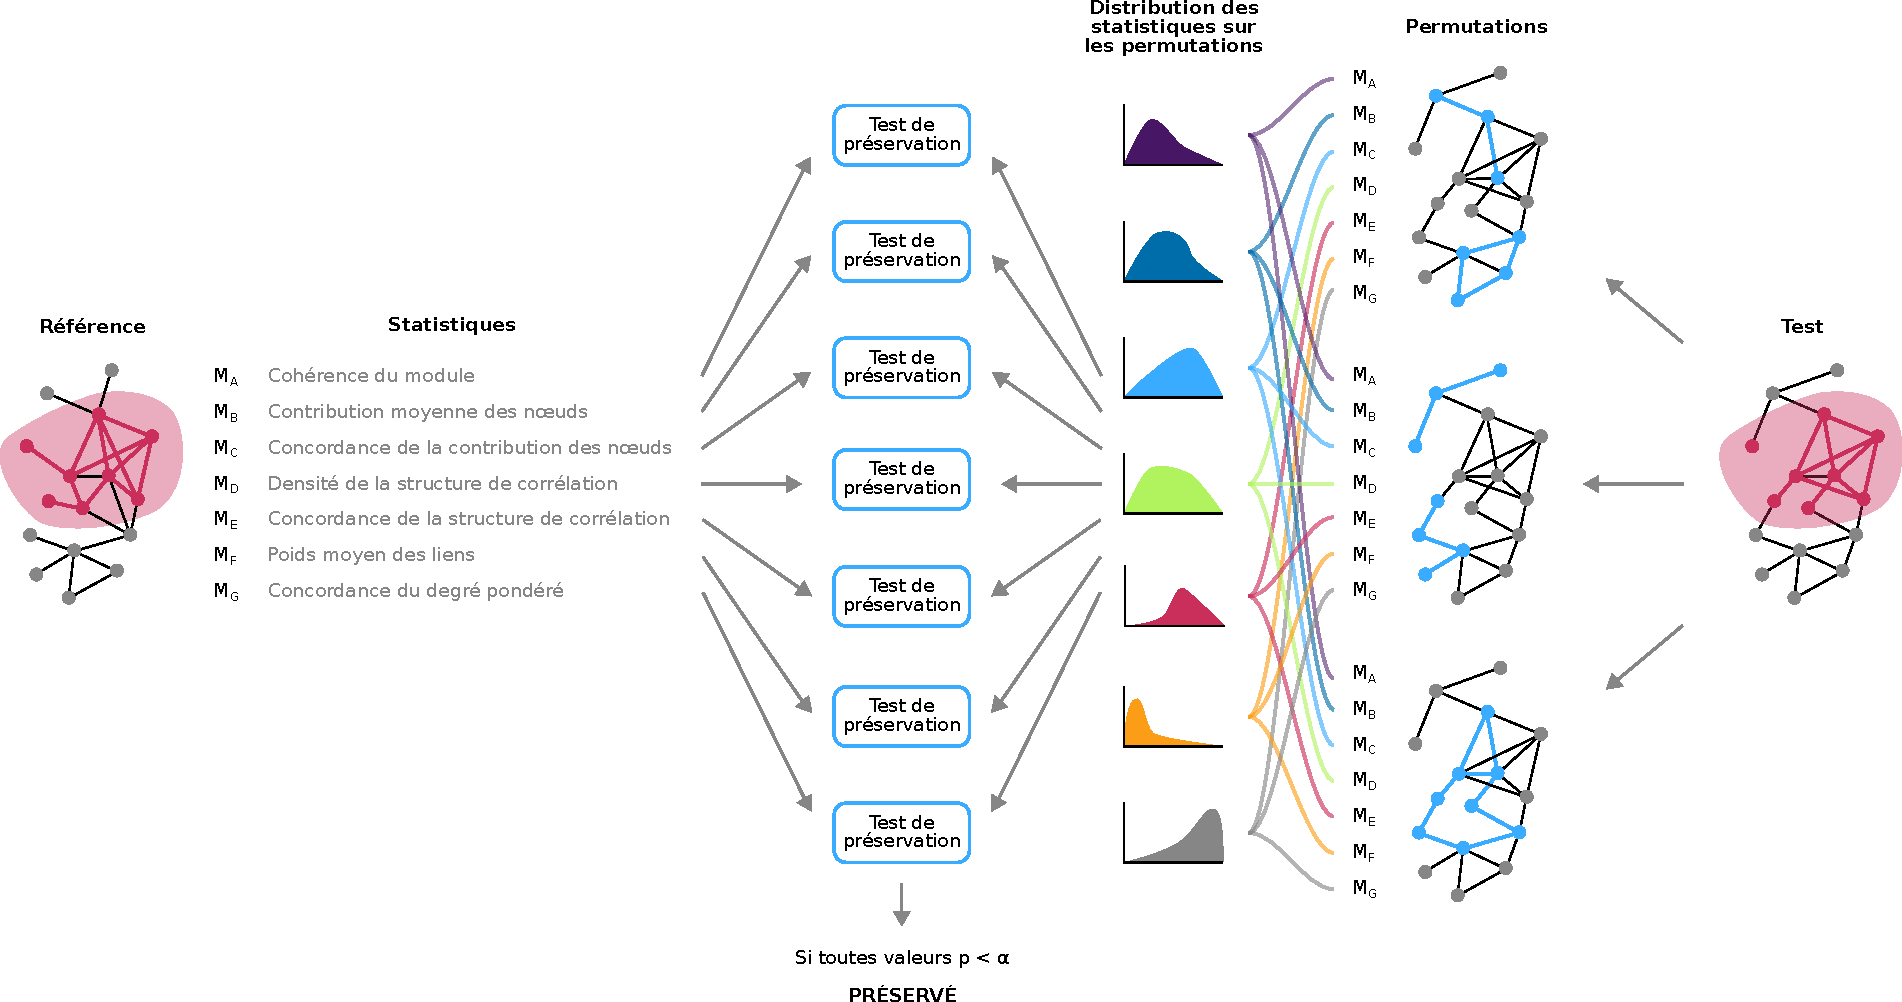
\includegraphics[width=\textwidth]{img/intro/3_coexpr/intro_3_coexpr_netrep_permut.pdf}
    \caption[Fonctionnement du test de permutation implémenté par S. Ritchie.]{Fonctionnement du test de permutation implémenté par S. Ritchie \cite{Ritchie2016}. Les réseaux construits dans chaque condition sont assignés d'un rôle : référence pour le réseau qui servira de contrôle, et test pour celui dans lequel sera vérifié la préservation du module. Le réseau de test est permuté plusieurs fois (minimum 1000 fois) et les sept statistiques sont calculées dans chacun pour finalement obtenir la distribution nulle du réseau. Un test de préservation est ensuite réalisé à l'aide des 7 statistiques calculées dans le réseau de référence et des distributions nulles. Si la totalité des sept valeurs p est significative, alors le module est dit préservé.}
    \label{fig:permutation_test}
\end{figure}

%%%%%% Discussion avec Leopold sur IRC pour détailler et comprendre le test de permutation de NetRep
%  Le soucis c'était de comprendre en quoi tester un evenement unique dans un réseau par rapport à une distribution nulle (générée par la randomisation des identifiants de noeuds dans le réseau) permettait de prouver la préservation. La réponse c'est que une seule stat ne permet pas de le prouver car t'as trop de degrés le liberté qui permettraient d'avoir une stat significative par hasard (sauf alpha giga strict). Donc ce qu'ils font c'est qu'ils calculent 7 stats qui caractérisent la topologie dans la condition controle, et qu'ils testent chacune sur la distribution nulle respective calculée sur tous les réseaux permuté. Ca contraint ton réseau test à respecter une topologie quasi identique pour remplir tous les critere, aka les 7 stats, et donc ca réduit la change d'avoir un réseau qui serait différent mais remplirait les 7 stats pareil que le reseau de controle
% Si je reprend ton analyse du rubix cube, c'est comme si on faisait 3 stats par face au niveau des couleurs (somme, moyenne, mediane des couleurs en RGB) et qu'on vérifiait si entre un rubix cube de controle et un rubix cube test, on retrouve ces 3 stats significatives sur 1000 permutations du rubix cube. À moins d'avoir un rubix cube avec le meme nombre de couleur et en meme proportion que le rubix controle, c'est très dur de faire dire la même chose aux 3 stats avec le rubix de test
% Et plus t'as de stats (non recoupantes) qui caractérisent ton rubix, plus tu réduit ta chance que le rubix test te nique par hasard

\section{Le vieillissement, une imbrication complexe de dérèglements}


Source multi-factorielle de changements dans l'\gls{organisme}, le vieillissement est, chez l'humain, un continuum de dérèglements conduisant une personne en bonne santé à une réduction de sa qualité de vie en raison d'une dégradation progressive des fonctions de base du corps \cite{Berrut2013}. Ses différents aspects ne forment pas un chemin linéaire mais plutôt une arborescence où chaque individu va tendre à accumuler plus ou moins plus vite certaines marques du vieillissement. Si certaines de ces marques n'impactent que légèrement la dégradation de la personne vieillissante ou âgée, des événements traumatiques ou pathologiques tels qu'un accident vasculaire cérébral peuvent, par un effet de cascade, entraîner une accélération brutale dans la vitesse de dégradation. En augmentant la \gls{longevite} des personnes, les avancées en santé publique et qualité de vie ont alors retardé la dégradation fonctionnelle. Paradoxalement, elles ont cependant augmenté l'âge maximal et donc l'accumulation des marques du vieillissement, rendant cette population plus susceptible à des maladies chroniques telles que le cancer ou les maladies cardiovasculaires \cite{Khan2017Aug}. 

\begin{figure}[ht]
    \centering
    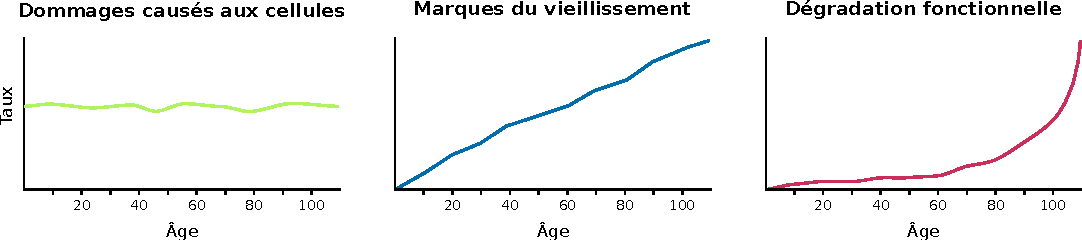
\includegraphics[width=\textwidth]{img/intro/4_aging/intro_4_aging_rate_marks.pdf}
    \caption[Lois de distribution régissant le vieillissement sous un modèle simplifié]{Lois de distribution régissant le vieillissement sous un modèle simplifié : l'exposition aux facteurs de vieillissement, l'accumulation cellulaire de dommages, l'augmentation exponentielle de la dégradation fonctionnelle et du risque de mortalité. Cette augmentation s'explique par le niveau constant de dommages causé aux cellules couplé à la réduction progressive des capacités de réparation qui est elle-même affectée par les dommages dans une boucle délétère \cite{Todhunter2018}.}
    \label{fig:aging_rate_marks}
\end{figure}

On distingue trois types de vieillissements : le vieillissement réussi ou en bonne santé, le vieillissement usuel, et le vieillissement pathologique \cite{vanBuchem2004Dec}. Le vieillissement réussi est décrit comme associé à l'absence de facteurs de risque pour la santé et avec une perte minime de condition physiologique : pas d'anomalies sanguines, pas de problèmes à l'effort, seulement un ralentissement de l'activité en raison d'une fatigue plus rapide \cite{Berrut2013}. Le vieillissement usuel est défini par une diminution des capacités fonctionnelles globales telles que visible en moyenne chez des personnes du même âge. Il implique les différents changements de régulation cellulaire et moléculaire qui vont se manifester à l'échelle de la personne par des déséquilibres métaboliques, des facteurs de risques augmentés, et des pathologies chroniques sans décompensation c’est-à-dire sans dégradation brutale suite à une rupture des \glspl{mecanisme} de compensation d'un dérèglement \cite{Berrut2013}. Enfin, le vieillissement pathologique est un terme ne faisant pas l'unanimité car étant un processus physiologique intrinsèque, il est discutable de le considérer comme une maladie. De ce fait, il est le plus souvent décrit comme recoupant deux notions : le vieillissement prématuré et le vieillissement en continuité avec le grand âge \cite{Belmin2014}. Tous ces vieillissements entretiennent évidemment des liens étroits d'un point de vue physiologique, mais on a souhaité dans cette thèse se concentrer sur le vieillissement usuel.


\subsection{Définition moléculaire}

% \todo[inline]{Retravailler avec la MAJ de Lopez-Otin par Ferruci 10.1111/acel.13080}

% Le vieillissement usuel, qu'on nommera simplement par la suite vieillissement, est influencé par la génétique d'un individu \cite{Khan2017Aug, deMagalhaes2003Mar} ainsi que son environnement \cite{Jones2015Dec}. C'est un phénomène inévitable qui ne reflète pas nécessairement l'âge chronologique d'un individu mais plutôt un âge biologique \cite{Horvath2013Oct}. 
Le vieillissement usuel, qu'on nommera simplement par la suite vieillissement, est inévitable et ne reflète pas nécessairement l'âge chronologique d'un individu mais plutôt un âge biologique \cite{Horvath2013Oct}. C'est un phénomène influencé par la génétique d'un individu \cite{Khan2017Aug, deMagalhaes2003Mar} ainsi que son environnement \cite{Jones2015Dec}. Des gènes associés à la longévité ont ainsi pu être identifiés mais sont loin d'expliquer la totalité du vieillissement au vu de sa très grande complexité moléculaire. Pour aider à la communication sur le sujet et pour tenter de catégoriser les différentes composantes du vieillissement, López-Otín \textit{et al.} proposent en 2013 un découpage en neuf \textbf{\glspl{aging_hallmarks}} du vieillissement (\textit{hallmarks of aging} en anglais) qui sont représentatives des causes, conséquences et résultats du vieillissement (Figure \ref{fig:hallmarks_aging}) \cite{Lopez-Otin2013} : 
% instabilité génomique, attrition des télomères, altérations épigénétiques, perte de protéostasie, dérégulation de la perception des nutriments, dysfonction mitochondriale, senescence cellulaire, épuisement des cellules souche, communication intercellulaire altérée. 
\begin{itemize}
    \item \textbf{Instabilité génomique} : l'intégrité de l'ADN est régulièrement mise à l'épreuve lors de la vie cellulaire, qu'il s'agisse de contraintes physiques, de conditions chimiques ou d'agents biologiques \cite{Moskalev2013Mar}. Ils entraînent des mutations ponctuelles, des translocations, des duplications et des augmentation ou réduction de taille de chromosome, notamment au niveau des télomères. Pour conserver sa stabilité, des mécanismes de stabilité et réparation de l'ADN sont présents dans la cellule mais tendent à dysfonctionner avec l'âge, permettant aux dommages de perdurer et se transmettre \cite{Lord2012Jan}. 
    \item \textbf{Attrition des télomères} : les télomères, extrémités des chromosomes, jouent un rôle de protection vis-à-vis de ceux-ci. Lors de la réplication cellulaire et en l'absence de télomérase dans la majorité des cellules, ils tendent toutefois à réduire en taille à chaque fois \cite{Lopez-Otin2013}. Leur taille initiale limite donc le nombre maximal de réplication qu'une cellule pourra avoir, nombre qui est appelé la limite de Hayflick \cite{Hayflick1961Dec}. Les télomères jouent donc un rôle dans la longévité globale mais peuvent être affectés par l'instabilité génomique ou des pathologies ponctuelles telles que des infections \cite{Ilmonen2008May}.
    
\begin{figure}[b]
    \centering
    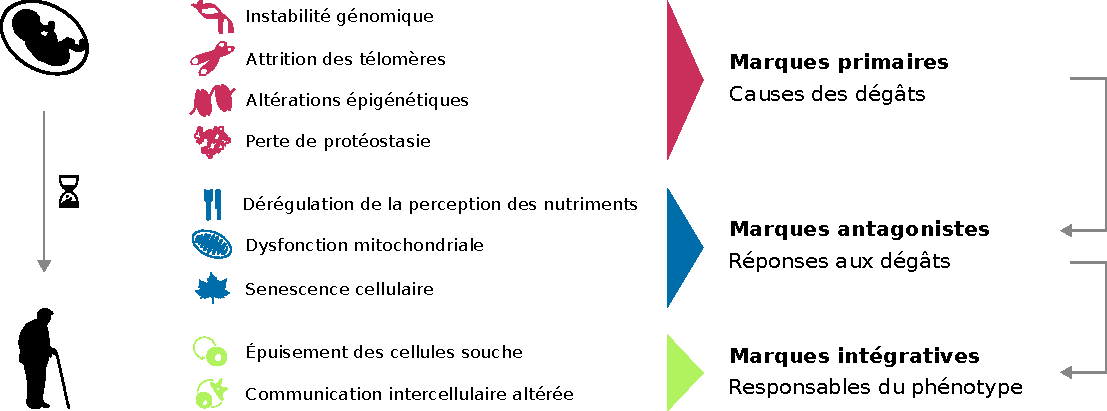
\includegraphics[width=\textwidth]{img/intro/4_aging/intro_4_aging_Lopez-Otin_hallmarks.pdf}
    \caption[Marques principales du vieillissement et interconnections fonctionnelles]{Marques principales du vieillissement et interconnections fonctionnelles. Adapté et traduit d'après López-Otín 2013 \cite{Lopez-Otin2013} \footnotemark. Les neuf marques principales proposées du vieillissement sont regroupées en trois catégories. (En haut) Les signes distinctifs considérés comme les causes primaires des dommages cellulaires. (Au milieu) Ceux qui sont considérés comme faisant partie des réponses compensatoires ou antagonistes aux dommages. Dans un premier temps, ces réponses atténuent les dommages, mais à terme, si elles sont chroniques ou exacerbées, elles deviennent elles-mêmes délétères. (En bas) Signes distinctifs intégratifs qui sont le résultat final des deux groupes de signes distinctifs précédents et sont finalement responsables du déclin fonctionnel associé au vieillissement.}
    \label{fig:hallmarks_aging}
\end{figure}

    \item \textbf{Altérations épigénétiques} : l'épigénétique désigne tout mécanisme de modification du génome n'incluant pas d'altération de sa séquence. Lors du vieillissement, plusieurs de ces mécanismes, comme la modification des histones chargés du repliement de la chromatine, vont entraîner des modifications de la régulation de la transcription \cite{Fraga2007Aug}. La perturbation de certaines voies comme la voie métabolique de l'insuline vont alors jouer sur la longévité des individus \cite{Jin2011Aug}.
    \item \textbf{Perte de protéostasie} : la protéostasie regroupe l'intégralité des mécanismes visant à permettre aux protéines d'acquérir et conserver leur repliement prévu, ainsi que les mécanismes de lyse des protéines pour éviter leur malfonctionnement en cas de dégâts \cite{Koga2011Apr}. Les liens précis entre les marques principales précédentes et la perte de protéostasie restent encore à comprendre malgré une association avérée de l'augmentation de mauvais repliement et de perte de proteolyse avec le vieillissement \cite{Koga2011Apr}.
    \item \textbf{Dérégulation de la perception des nutriments} : la perception des fluctuations des niveaux de nutriments dans l'\gls{organisme} telles que les sucres, acides aminés, et lipides est essentiel pour son fonctionnement et requière différentes voies d'activation spécifiques à chacun \cite{Houtkooper2010Jul}. Face à la déficience de régulation de nutriments chez les personnes âgées, il a été observé que plusieurs voies tendent à être perturbées, par exemple mTOR dans la perception des hautes concentrations en acides aminés \cite{Laplante2012Apr}.
    \item \textbf{Dysfonction mitochondriale} : les mitochondries, organelles chargées entre autre de la respiration cellulaire, diminuent en activité avec le vieillissement ce qui cause un ralentissement de croissance \cite{Green2011Aug}. La production d'adénosine triphosphate (ATP) nécessaire aux nombreuses réactions cellulaires décroit donc et avec elle le métabolisme global de la cellule. Des dérivés réactifs de l'oxygène (en anglais \textit{reactive oxygen species} ou ROS) sont également mesurés en plus grande quantité en conséquence, bien que leur rôle soit ambigu. Il a été observé que leur présence tend dans certains contextes à stimuler des réponses de compensations du vieillissement qui augmentent la longévité, et dans d'autres contextes à diminuer la longévité en raison du stress cellulaire induit \cite{Ziegler2015Feb}.
    \item \textbf{Sénescence cellulaire} : la duplication cellulaire fait partie de la vie normale d'une cellule et se retrouve arrêté de façon stable dans un processus qu'on nomme sénescence. Plusieurs mécanismes peuvent mener la cellule à ce stade tel que le raccourcissement des télomères précédemment cité. D'autres formes de sénescence existent toutefois sous la forme de sécurités mises en place par la cellule pour éviter la multiplication de cellules atteintes par des dommages conséquents à l'ADN \cite{Khan2017Aug}. Ces cellules sénescentes sont également connues pour contribuer à une inflammation chronique de faible intensité (en anglais \textit{inflammaging}) \cite{Kuilman2010Nov,Franceschi2014} et leur signalisation pro-sénescence à travers les différents tissus \cite{Khan2017Aug}.
    \item \textbf{Épuisement des cellules souche} : la réduction des capacités de différenciation et régénération des cellules souches sont la conséquence des altérations des dommages à l'ADN et des mécanismes de sénescence en réponse pour limiter leur prolifération \cite{Sharpless2007Sep}. En atteignant par exemple les niches de cellules souches telles que celle des cellules hématopoïétiques, les dommages à l'ADN et à la régulation vont causer une diminution des capacités immunitaires (aussi appelée immuno-sénescence) ainsi qu'une anémie \cite{Lopez-Otin2013,Baker2016Feb}.
    \item \textbf{Communication intercellulaire altérée} : les dérégulations de l'\glspl{genexpr} couplés à des stimulations de faible intensité du système immunitaire entraînent un brouillage de la communication entre cellules par diverses sécrétions dans la matrice extra-cellulaires \cite{Lopez-Otin2013}. Le système endocrinien comme paracrinien vont voir leurs capacités de coordination du métabolisme entre cellules réduites, ce qui va à son tour mener à des dommages dans l'ADN des cellules \cite{Khan2017Aug}. Ce phénomène peut s'accentuer localement au point d'engendrer un vieillissement accéléré d'un tissu qui peut promouvoir la sénescence dans d'autres tissus au point qu'on le nomme vieillissement métastatique \cite{Lavasani2012Jan}.
\end{itemize}
\hfill


Comme visible dans ces définitions ainsi que dans la Figure \ref{fig:hallmarks_aging}, plusieurs de ces marques principales du vieillissement tendent à s'entretenir les unes les autres dans un cercle vicieux s'accentuant à chaque cycle. Des mécanismes de compensations visent toutefois à contrer ce cycle en stoppant les cellules atteintes par la senescence, ou en re-stimulant leur régénération comme cela a pu être vu avec les ROS. Ces mécanismes sont d'ailleurs présents avant l'apparition du vieillissement qui n'est finalement qu'une illustration de la mise en échec progressive de la robustesse des mécanismes de compensation \cite{Ferrucci2020Feb}.

\footnotetext{Texte requis par l'éditeur : Cette traduction n'est pas officielle et n'a pas été approuvée par Elsevier}


% GWEN ! LÀ STOP ! MAJ DE LOPEZ-OTIN : https://onlinelibrary.wiley.com/doi/epdf/10.1111/acel.13080


\subsection{Enjeux}

Si la quête pour l'immortalité a su inspirer nombre de personnes et de récits, elle n'est pas souhaitable pour plusieurs raisons tant éthiques qu'économiques \cite{Hayflick2000}. Il n'est donc pas question de guérir ou empêcher le vieillissement dans le cadre de la recherche sur celui-ci mais de le comprendre. L'âge entraîne la multiplication des facteurs de risque et est associées à des maladies lui étant quasi spécifiques comme la maladie d'Alzheimer, l'athérosclérose, le cancer, l'insuffisance rénale chronique, l'obstruction pulmonaire chronique, l'insuffisance cardiaque, l'ostéoporose, la maladie de Parkinson, la sarcopénie, et le diabète de type 2 \cite{Kubben2017}. Leur fréquence dans la population a d'ailleurs augmenté depuis plusieurs années et va continuer d'augmenter puisque la part d'humains dépassant les 65 est supérieure aujourd'hui à celle des moins de 5 ans et qu'elle croît encore \cite{Phillips2021Apr}. 

De la fragilité qu'engendrent ces maladies du vieillissement découlent de nombreuses contraintes physiques, économiques et sociales \cite{Blasimme2017Feb}. Face à la fatigue et la réduction de tonus corporel, les personnes âgées vont perdre progressivement en autonomie et nécessiter un accompagnement de plus en plus systématique par des structures d'aide à la personne et de soin chronique. L'augmentation de l'affluence de personnes à prendre en charge dans les années à venir va donc représenter un défi pour le système de santé publique \cite{Phillips2021Apr}. Si l'option d'augmenter les capacités hospitalières et sociale existe, il serait moins coûteux de chercher à prévenir le vieillissement. La recherche actuelle vise donc à comprendre le vieillissement, non pas pour augmenter la longévité, mais plutôt pour contrer à la racine ses effets néfastes pour finalement vieillir en bonne santé \cite{Ferrucci2020Feb}.

% Transition commencée mais pas adaptée car c'est la transcripto après et pas les enjeux de ma thèse
% Les connaissances actuelles pointent sur différents points d'action pour contrer le vieillissement, thérapeutiques ou préventifs.



% \subsection{La capture de l'information liée au vieillissement par la transcriptomique}
\subsection{L'étude du vieillissement à travers les réseaux de co-expression}

Le vieillissement va directement impacter l'\glspl{genexpr} en raison des dérégulations causées. Les différentes marques principales du vieillissement seront donc perceptibles, chacune dans une mesure variable, à travers l'étude du \gls{transcriptome} \cite{Saint2020Jun}. Ce profilage \gls{transcriptomique} a permis par le passé l'identification de nombreux biomarqueurs uniques ou combinés associés à une marque principale du vieillissement ou à la longévité \cite{Melzer2020}. Les bases de données \textit{GenAge} \cite{DeMagalhaes2004} et \textit{Digital Aging Atlas} \cite{Craig2015} répertorient ainsi respectivement 307 gènes humains avérés associés au vieillissement et 2599 gènes humains impliqués dans des variations lors du vieillissement ou de la longévité. Une étude réalisée par de Magalhães \textit{et al.} identifie toutefois seulement 73 gènes constamment associés avec le vieillissement \cite{DeMagalhaes2009intro}. Les autres gènes présents dans ces différentes bases de données présentent des gènes variant spécifiquement dans un tissu, un sexe, ou en présence d'une maladie spécifique du vieillissement. Ils vont par ailleurs, pour une même marque principale du vieillissement comme le raccourcissement des télomères, avoir une manifestation différente entre tissus en raison de leur fonction ou leur taux de renouvellement (Table \ref{table:tissu_telomere_effet}).

\begin{table}[hb]
\resizebox{\textwidth}{!}{
\begin{tabular}{m{0.2\textwidth}m{0.2\textwidth}m{0.6\textwidth}}
\textbf{Type de tissu}                                                                    & \textbf{Nom du tissu}                                            & \textbf{\begin{tabular}[c]{@{}l@{}}Manifestations pathologiques chez l'humain \\ avec syndromes télomériques\end{tabular}} \\ \hline
\multirow{4}{*}{\begin{tabular}[c]{@{}l@{}}Tissus à fort\\ renouvellement\end{tabular}}   & Peau                                                             & • Blanchissement prématuré des cheveux                                                                                     \\
                                                                                          & \begin{tabular}[c]{@{}l@{}}Moelle \\ osseuse\end{tabular}        & • Anémie aplastique                                                                                                        \\
                                                                                          & Immune                                                           & \begin{tabular}[c]{@{}l@{}}• Infections opportuniste\\ • Immunodéfiscience des cellules B, T et NK\end{tabular}            \\
                                                                                          & \begin{tabular}[c]{@{}l@{}}Épithélium \\ intestinal\end{tabular} & \begin{tabular}[c]{@{}l@{}}• Entérocolite\\ • Émoussement villositaire\end{tabular}                                        \\
\multirow{3}{*}{\begin{tabular}[c]{@{}l@{}}Tissus à faible\\ renouvellement\end{tabular}} & Poumon                                                           & \begin{tabular}[c]{@{}l@{}}• Emphysème prématuré\\ • Fibrose pulmonaire idiopathique\end{tabular}                          \\
                                                                                          & Foie                                                             & • Fibrose-cirrhose du foie cryptogénétique                                                                                 \\
                                                                                          & Os                                                               & \begin{tabular}[c]{@{}l@{}}• Ostéoporose\\ • Nécrose avasculaire\end{tabular}                                              \\
Cancer                                                                                    & Multi-tissus                                                     & \begin{tabular}[c]{@{}l@{}}• Cancers épithéliaux\\ • Hémopathies malignes\end{tabular}                                    
\end{tabular}
}
\caption[Phénotypes de maladies spécifiques aux organes si télomères courts]{Phénotypes de maladies spécifiques aux organes chez les humains ayant des télomères courts. Modifié d'après la Table 2 de Armanios 2012, \textit{The telomere syndromes} \cite{Armanios2012}}
\label{table:tissu_telomere_effet}
\end{table}

Le vieillissement est une imbrication simultanée et complexe de plusieurs altérations de l'intégrité des cellules. Ces gènes associés au vieillissement et agissant comme biomarqueurs ne permettent pas à eux seuls de comprendre quelles sont les voies métaboliques qui sont impactée et comment ces gènes vont contribuer à d'autres altérations. 
Les \acrshort{GCN} sont alors particulièrement adaptés pour répondre à ce besoin grâce à l'étude des \glspl{voisin} de ces biomarqueurs \cite{delaFuente2010Jul}. Par l'étude des modules détectés dans leurs réseaux, il est également possible de détecter de nouveaux biomarqueurs, soit en analysant la topologie de modules associés au \gls{phenotype} de l'âge, soit en effectuant une analyse de co-expression différentielle entre plusieurs tranches d'âge et en isolant les gènes responsables de la non-préservation des modules \cite{Zierer2015}. Il serait également possible d'effectuer cette co-expression différentielle entre tissus, espèces, populations pour estimer la part de spécificité et la part commune de vieillissement.

En 2009, les \acrshort{GCN} vont même permettre de venir compléter l'idée de la désorganisation de la transcription dans le vieillissement. En observant différents tissus entre des souris de 16 et 24 mois, Southworth \textit{et al.} vont mettre à jour un phénomène de perte de densité de co-expression avec l'âge \cite{Southworth2009}. Plus précisément encore, ils vont démontrer que cette perte n'est pas uniforme, mais se fait de façon modulaire, probablement en raison d'une colocalisation sur un chromosome des gènes impliqués. Ce phénomène sera d'ailleurs retrouvé dans de nombreuses études sur les cancers, ensemble de maladies connu pour partager plusieurs marques principales du vieillissement \cite{Anglani2014}. Peu d'études sur ce phénomène ont suivi dans le cadre du vieillissement et une exploration plus détaillée de cette perte chez l'homme et sur plusieurs points dans l'âge d'un \gls{organisme} sont à envisager.



% Aide à la justification de l'utilisation de la co-expression dans l'étude du vieillissement :  Next-generation sequencing in aging research: Emerging applications, problems, pitfalls and possible solutions 10.1016/j.arr.2009.10.006
% Inflammaging and Garb-aging : https://www.sciencedirect.com/science/article/abs/pii/S1043276016301254
%% Transcription and Aging (book) : https://doi.org/10.1007/978-981-32-9005-1_3
%% The aging transcriptome: read between the lines : https://www.sciencedirect.com/science/article/abs/pii/S0959438820300878
%% Modeling the human aging transcriptome across tissues, health status, and sexhttps://onlinelibrary.wiley.com/doi/abs/10.1111/acel.13280

% Intro potentielle (A RETRAVAILLER)
% De Magalhães s'interrogeait en 2003 \cite{deMagalhes2003} d'une potentielle programmation génétique du vieillissement. Il voyait comme perspective de cette question de recherche une compréhension du vieillissement et donc une façon pérenne de retarder d'un seul coup l'apparition de quelques, si ce n'est toutes, maladies chez la personne âgée.
% % La question sous-jacente abordée était finalement de savoir si analyser et comprendre indépendamment chaque conséquence néfaste et maladie apparaissant avec l'âge n'était pas une course perdue d'avance pour les combattre. Ainsi, De Magalhães envisageait que comprendre le fonctionnement global du vieillissement serait plus pérenne pour retarder d'un seul coup l'apparition de quelques, si ce n'est toutes, maladies chez la personne âgée.







\section{Motivations et hypothèses de recherche}

Face à la sous-exploitation des \acrshort{GCN} dans l'analyse \gls{transcriptomique} et à leur potentiel dans l'étude du vieillissement, j'ai souhaité faciliter l'accès à cette méthode et démontrer plusieurs aspects sur lesquels elle est à même d'aider. Les outils dédiés aux \acrshort{GCN} existant au début de cette thèse présentaient de nombreux frein à l'utilisation par des utilisateurs sans formation en bioinformatique et biostatistique ou par des utilisateurs souhaitant faire une analyse rapide clef en main. Ces outils n'utilisaient également pas le potentiel d'un assemblage de logiciels façon pipeline, et si certains outils s'en inspirant ont été publiés durant cette thèse, aucun d'entre eux ne considérait la pérennité de l'outil final dans leur architecture implémentée.

Cette thèse a donc été le siège de deux hypothèses de recherche. La première consistait à s'interroger sur la faisabilité d'un outil pipeline sous la forme d'un progiciel R déposé sur Bioconductor qui tirerait parti des outils existants pour chaque étape de l'analyse de co-expression et prévoirait la possibilité de les remplacer dans le futur par d'autres grâce à une architecture logiciel modulaire. La seconde supposait que l'utilisation d'un tel outil pourrait permettre de faciliter la découverte de nouveaux biomarqueurs spécifiques et communs du vieillissement entre différents tissus humain via des réseaux construits chacun. Chacune de ces hypothèses a donc été testée au cours de cette thèse dans un chapitre qui lui est dédié.



% ###########################################################################################################

% CONTENU SUPPLÉMENTAIRE AU BESOIN :
% 
% Phrases 
% - "Studies have shown that each gene is estimated on average to interact with four to eight other genes1 and to be involved in 10 biological functions" [10.1038/s41598-017-18705-z]
% - "A very clear partition of different biological networks is provided by Christensen et al. [1], who separated these networks into five main categories as follows: [metabolic networks, signal transduction networks,transcriptional regulatory networks, protein-protein networks, functional gene networks]" [10.1093/bfgp/elt003]
% - "It has been reported that nearly one in four studies uses public data to address a biological problem without generating new raw data (Rung and Brazma, 2013)." [10.3389/fpls.2016.00444]
% 
% Liens 
% - The human transcriptome, an unfinished story  https://www.mdpi.com/2073-4425/3/3/344/htm
% - Infos sur la peau : these super interessante => https://dumas.ccsd.cnrs.fr/dumas-01599807/document% 
% - "Two evolutionary theories of ageing — the mutation-accumulation and trade-off theories "
% -  The future of ageing https://www.nature.com/articles/35041709
% - Bouquin vieillissement https://library.oapen.org/bitstream/handle/20.500.12657/24382/1005732.pdf?sequence=1#page=98
% - https://www.nature.com/articles/nrm.2017.68 maladies définies comme associées à l'âge
% - ACcumulation erreurs et lien avec la mortalité (page 123) https://www.sciencedirect.com/science/article/abs/pii/S095506741730131X
% - Age dependant/independant mortality : https://en.wikipedia.org/wiki/Gompertz%E2%80%93Makeham_law_of_mortality
% - REview biomarqueurs et forces d'action sur le vieillissement : https://sci-hub.se/10.1007/978-3-030-25650-0

